\chapter[A Lighthouse in the Dust]{Reverberation of Doppler Boosted Emission from Massive Black Hole Binaries I: A Lighthouse in the Dust}
\label{ch:Dust}
\let\thefootnote\relax\footnotetext{Draft Version May 24, 2016: We dedicate this work to the memory of Arlin Crotts who passed away on November 19, 2015.}





% \documentclass[usenatbib]{mnras}



% \newcommand\lsim{\mathrel{\rlap{\lower4pt\hbox{\hskip1pt$\sim$}}
%         \raise1pt\hbox{$<$}}}
% \newcommand\gsim{\mathrel{\rlap{\lower4pt\hbox{\hskip1pt$\sim$}}
%         \raise1pt\hbox{$>$}}} 
        
% \usepackage{amsmath}
% \usepackage{float}

% %%% Ion species with small caps.
% %\newcommand\ion[2]{#1{\thinspace\scshape#2}}% 

% \usepackage[usenames, dvipsnames]{color}
% % graphicx is for figures
% \usepackage{graphicx}
% % verbatim is for comment environment                                           
% \usepackage{verbatim}

% % hyperlink references
% \usepackage{hyperref}
% \hypersetup{
%     pdfnewwindow=true,      % links in new window
%     colorlinks=true,       % false: boxed links; true: colored links
%     linkcolor=blue,          % color of internal links
%     citecolor=cyan,        % color of links to bibliography
%     filecolor=blue,      % color of file links
%     urlcolor=blue           % color of external links
% }



% %%% Journal abbreviations.
% \def\prd{PRD}
% \def\apj{ApJ}                 % Astrophysical Journal
% \def\apjl{ApJL}               % Astrophysical Journal, Letters
% \def\apjs{ApJS}               % Astrophysical Journal, Supplement
% \def\mnras{MNRAS}             % Monthly Notices of the RAS
% \def\aap{A\&A}                % Astronomy and Astrophysics
% \def\aaps{A\&AS}              % Astronomy and Astrophysics, Supplement 
% \def\aj{AJ}                   % Astronomical Journal
% \def\physrep{Phys.~Rep.}      % Physics Reports
% \def\nat{Nature}              % Nature
% \def\araa{ARA\&A}             % Annual Review of Astronomy and Astrophysics
% \def\planss{planss}           % Planetary and Space Science
% \def\ssr{SSR}                 % Space Science Reviews          
% \def\sovast{Sov.~Astron.}     % Soviet Astronomy         
% \def\canjphys{Can. J. Phys.}  % Canadian Journal of physics
% \def\actaa{Acta Astron}  % Acta Astronomica  - polish astronomy and astrophysics
% \def\icarus{Icarus}  % Solar System studies journal

% % Math Definitions
% \newcommand{\scripty}[1]{\ensuremath{\mathcalligra{#1}}}
% \def\sr{\scripty{r}}
% \def\Mach{\mathcal{M}}
% \def\bin{\rm{bin}}
% \def\sky{\rm{s}}
% \def\orb{\rm{orb}}
% \def\obs{\rm{obs}}
% \def\eff{\rm{eff}}
% \def\Rout{R_{\rm{out}}}
% \def\Rin{R_{\rm{d}}}
% \def\em{\rm{em}}
% \def\Mdot{\dot{M}}
% \def\Msun{ M_{ \rm{\odot} } }



% \begin{document}
% \begin{onecolumn}

% \title[]{Reverberation of Doppler Boosted Emission from Massive Black Hole Binaries I: A Lighthouse in the Dust\footnote{We dedicate this work to the memory of Arlin Crotts who passed away on November 19, 2015. As an expert on supernovae light echoes, we sorely missed his collaboration on this work.}} 

% \author[D. J. D'Orazio, Z. Haiman]{Daniel J. D'Orazio$^1$, Zolt\'an~Haiman$^1$  \\
%     %\thanks{dorazio@astro.columbia.edu; zoltan@astro.columbia.edu}\\
%      $^1$Department of Astronomy, Columbia University, 550 West 120th Street, New York, NY 10027 }

% \maketitle



% \begin{abstract} 
% We consider the reverberation of AGN emission by dust in the
% context of massive black hole binaries which emit periodic continuum emission
% due to both spatially isotropic variations and anisotropic variations caused by orbital relativistic Doppler boosting. We develop a toy model for infrared
% emission from AGN harboring such MBHBs, providing an additional test to vet
% the Doppler boosting model for MBHB candidates, and a tool for constraining properties of the
% dusty environments around MBHBs. We determine that, in the Doppler boost model, IR variability and optical/UV variability need not be coincident. Depending on the relative inclinations of the binary plane, observer, and dust torus, as well as the ratio of binary orbital period to the light travel time from source to dust, UV emission could be steady, while the IR is periodically modulated, or vice versa. IR surveys should look for such orphan IR variability.
% %
% %We find that, in the Doppler boost model, the phase and magnitude of the reverberated IR light curve can depend heavily on the binary inclination and orbital period relative the the surrounding dust geometry and radius. From study the IR light curve dependence on binary and dust parameters, we conclude that IR variability searches may be fruitful in identifying MBHB candidates  
% We apply our models to the WISE data for
% infrared emission from MBHB candidate PG 1302. Assuming a
% smooth torus model for the dust around PG 1302, and assuming the dust is optically thin to its own emission, we find best fit models for isotropic and Doppler boost models, finding that both can capture the average magnitude, phase lag, and variability amplitude of the IR emission in the W1 and W2 WISE bands. 
% %
% %The Doppler scenario, however, formally provides a better fit that the isotropic emission model. 
% %
% In the near future these model will help to corroborate evidence
% for the growing number of (presently $\gsim 100$) MBHB candidates, find new candidates, and also
% constrain their physical properties and the properties of their
% surrounding, dusty environments. 

% %our best fit model requires a
% %dust torus with opening angle $XX^{\circ} \pm XX^{\circ}$, an inclination to
% %the line of site of $XX^{\circ} \pm XX^{\circ}$, an inner torus radius
% %consistent with sublimation of Graphitic dust grains ($X.X \pm X.X$ pc), and a
% %total dust mass of $X.X \pm X.X \Msun$. In the future this model will help to corroborate evidence
% %for the growing number of (presently $\gsim 100$) MBHB candidates and also
% %constrain their physical properties as well as the properties of their
% %surrounding, dusty environments. 
% %
% %
% % %Main Results:  %1) The phase lag of the IR
% %curve is dependent not only on the size of the emission region, but also on
% %many other factors such as the geometry and orientation of the dust torus as
% %well as the relative pattern speed of the variable illuminating source.  
% %2) This toy makes predictions consistent with the measured IR light curves for PG
% %1302 and can constrain dust properties as well as binary parameters.  
% %(3) Even if UV optical modulation is not visible because of binary orbital
% %inclination, the IR modulation could still be! should do surveys with IR! WIse
% %only 40 are modulated? Future work - how many could be pop stats from UV vs IR
% %candidates! 
% %(4) The mass ratio is not as limited for Doppler signatures in the IR... 
% \end{abstract}


\section{Introduction} Massive black holes (MBHs) exist at the centers of
most, if not all, galaxies \citep{KR95, KormendyHo2013}. Galactic mergers can
deliver MBHs, as well as an ample supply of gas \citep{BH1992, Barnes:1996,
Barnes:2002, Mayer:2013:MBHBGasRev}, to the centers of newly coalesced
galaxies where the BHs form a binary. The interaction of massive black hole
binaries (MBHBs) with gas and surrounding stars can drive the pair to sub-pc
separations where gravitational radiation reaction drives the binary to
coalescence \citep{Begel:Blan:Rees:1980}.  Characterization of the population
of such sub-pc binaries, through present electromagnetic (EM), and future
gravitational wave (GW) channels will provide a powerful tool for
understanding the mutual build-up of galaxies and central black holes
\citep[\textit{e.g.}][]{KormendyHo2013}, the dynamics of gas and stars in
galactic nuclei \citep[\textit{e.g.}][]{MerrittMilos:2005:LRR}, and the low-
frequency gravitational wave background
\citep[\textit{e.g.}][]{KocsisSesana:2011, Shannon:2015,
Arzoumanian:2015:SGWB}.

The electromagnetic signatures of MBHBs can arise from their interaction with
gas. Hydrodynamical simulations of gas discs surrounding close MBHBs show that
accretion rates onto a binary can rival, and even exceed the accretion rates
onto a single black hole of an equivalent mass \citep{ShiKrolik:2012,
DHM:2013:MNRAS, Farris:2014, ShiKrolik:2015, MunozLai:2016}. Binary accretion
rates can also be uniquely identifiable. Depending on the ratio of BH masses,
$q \equiv M_2/M_1$ ($M_1>M_2$), the accretion induced emission can be
periodically modulated \citep{Farris:2015:Cool}. For systems with $q \gsim
0.05$, the accretion rate is modulated by the strong perturbations from the
time-dependent binary potential \citep{D'Orazio:CBDtrans:2016}. Periodicity in
the accretion rate, and the resulting luminosity of emission, occur at the
binary orbital period and also twice this period for $0.05 \lsim q \lsim 0.3$.
while for $0.3 \lsim q < 1.0$, an additional periodicity appears at $\sim3
\rightarrow 8\times$ the binary orbital period \citep{ShiKrolik:2012,
DHM:2013:MNRAS, Farris:2014, ShiKrolik:2015, MunozLai:2016}.

In addition to luminosity variations that track accretion rate variability,
luminosity variations will occur due to special relativity alone. For binary
components moving at relativistic speeds (greater than a few $\%$ the speed of
light), any emission will vary in brightness at the period of the binary orbit
due to Doppler Boosting \citep{PG1302MNRAS:2015a,
PG1302Nature:2015b}.\footnote{For equal mass binaries on circular orbits, each
BH emits at the same luminosity and moves at the same orbital speed, hence
Doppler boosting effects are nullified unless one BH can accrete at a higher
rate than the other; such a scenario may occur for eccentric binaries
\citep{MunozLai:2016}.}  For binaries with disparate mass ratios, $q \lsim
0.05$, accretion is steady and dominated by the smaller, secondary BH
\citep{DHM:2013:MNRAS, Farris:2014}. In this case Doppler Boosting is expected
to be the primary, if not only, source of variability. Even near-equal mass
binaries, for which high levels of accretion variability are expected, may
emit steadily in their rest frame: If viscous and tidal forcing timescales
which transport matter from the edges of the mini-disks around each BH down to
the BH inner most stable circular orbit are long compared to accretion rate
changes at the mini-disc edges, then luminosity variations may be muted by
buffering in the mini-disks. In this case too, Doppler boosting will be the
dominate source of variability from accreting MBHBs.



The Doppler boosting scenario has recently been developed to interpret the
MBHB candidate PG 1302-102 \citep{Graham+2015a}, which exhibits a nearly
sinusoidal periodicity in the V-band continuum. Given the measured binary
mass, period, and spectral slope of PG 1302, \cite{PG1302Nature:2015b} showed
that the observed amplitude of variability in the V-band and UV wavelengths is
consistent with that expected for Doppler boosting of light from an accretion
disk around the secondary BH. Further confirmation of the Doppler boosting
model for PG 1302 will require continued, long-term observations of the system
in optical and UV wavelengths, however measurements in other wavelengths can
provide additional clues to the nature of the central engine of PG 1302.

Such clues have recently come from the infrared (IR). \cite{Jun:2015}
(hereafter J15) analyze data from the WISE satellite to report a periodicity
in the IR continuum of PG 1302 which is consistent with the optical period,
but with a diminished amplitude and at a phase lag of $335 \pm 153$ days in
the W1 band and $524 \pm 148$ days in the W2 band. J15 attribute this phase
lag to reprocessing of the optical/UV continuum of PG 1302 by a surrounding
dusty torus at $\sim$pc distances from the illuminating source.

In this work we develop a toy model to interpret the findings of J15 and, in
general, reverberated IR emission from MBHBs. We considers heating of  nuclear
dust by isotropically varying emission from the central source, and compare to
models with spatially, and temporally, varying Doppler boosted binary
emission, illuminating the dust structure as it sweeps around like a
lighthouse at the binary orbital frequency. We crucially take into account the
relative light travel time to different parts of the dust structure and the
dust optical depth in a smooth, dusty- torus model. We find that the relative
magnitude and phase lag of the reverberated IR emission is dependent not only
on the size of the dust region, but also on its geometry and the pattern speed
of the variable illuminating source (the binary orbital period relative to the
light travel time to the dust region). We find also that, for Doppler boosted
emission models, depending on the relative inclination angles of the binary
and the dust torus to the observer's line of sight, variability can be present
in both optical and IR, or in one band and not the other. This means that
present optical surveys of MBHB candidates may have missed some candidates
which vary only in the reverberated IR and motivates and IR plus optical
search for periodic Quasars.

We apply both isotropic and Doppler boost models to fit the IR light curves
of MBHB candidate PG 1302. We find that both dust reverberation models can
consistently account for the observed IR emission. %with a preference for the Doppler boost scenario. 
Our model not only provides more evidence for the
Doppler boost explanation of PG 1302, but it also promises to constrain binary
parameters with future data as well as constrain the geometry and make-up of
the surrounding dust. The generic nature of this toy model will also allow us
to vet the Doppler boosting scenario for the new population of $\gsim100$ MBHB
candidates \citep{Graham+2015b, Charisi+2016} and probe their dusty
environments.

This work is organized as follows. In \S \ref{S:Model} introduce the MBHB and
dust system. In \S \ref{S:Derivation} we develop models for infrared emission
from a dust region heated by both isotropic and Doppler boosted MBHB
continuum, for a variety of different dust geometries and assumptions. In \S
\ref{S:PDs} we explore the parameter dependencies in the model,
differentiating between isotropic and Doppler boost scenarios. In \S
\ref{S:PG1302} we apply our models to the infrared data for MBHB candidate PG
1302, finding best fit binary and dust parameters. In section
\ref{S:Discussion} we consider limitations and future extensions to the model,
and conclude.





\section{Model Setup}
 \label{S:Model}
 \subsection{The Dust}

The unification of type I (unobscured) and type II (obscured) active galactic
nuclei (AGN) posits that the difference in AGN types is only the viewing angle
relative to a torus of obscuring dust \citep{Antonucci:1993,
KrolikBegelman:1988}. The properties of AGN dust have been investigated from
high resolution IR imaging as well as modeling of IR spectral energy
distributions (SEDs). High resolution IR imaging puts an upper limit of a few
parsecs on the size of the emitting dust region \citep[see][and references
within]{Elitzur:2006}. Spectral energy distribution (SED) modeling has put
forth a wide variety of models of optically thin and optically thick, smooth
and clumpy dust distributions of various geometries in order to determine dust
spatial distributions and dust grain size distributions  \citep[see the review by][as well as  \cite{Barvainis:1987,PierKrolikI:1992b, PierKrolikII:1993, LaorDraine:1993, GranatoDanese:1994,  Granato:1997,RowanRobinson:1995,Manske:1998,Nenkova:2002,vanBemmelDullemond:2003, Schartmann:2005, NenkovaI:2008,NenkovaII:2008, HonigII:2010, MorTrakhtenbrot:2011,MorNetzer:2012}]{Netzer:2015:rev}. Neither imaging or SED fitting, however, uniquely determine the dust properties.

%, but from these endeavors, a generic picture arises of a clumpy torus of dust surrounding the central AGN luminosity source. 


%In this work we demonstrate the effects of an anisotropic and periodically variable continuum source on reverberated IR light curves. 

We do not hope to reproduce the full SEDs of AGN dust tori. Instead we aim to
demonstrate the effects of an anisotropic and periodically variable continuum
source on the reverberated IR continuum. Hence, for simplicity, we assume a
smooth dust distribution of uniform size grains requiring only that the
density be monotonically decreasing away from the central source and
distributed in a torus geometry (see below). We work in both the optically
thin and optically thick limits.

%We proceed by considering the reprocessing of light from a central source of optical and UV continuum by a smooth dusty torus with the above, simplified properties.


%The dust grain size distribution can be included as a free parameter, and the global density distribution can be easily modified within our model. The inclusion of dust emission and absorption features \citep[\textit{e.g.} $9.7 \mu$m and $18 \mu$m emission silicate features][]{} could be included with further radiative transfer modeling. We proceed by considering the reprocessing of light from a central source of optical and UV continuum by a smooth dusty torus with the above, simplified properties.






%Optically thin models:
%\begin{enumerate}
%\item LaorDraine:1993 (also consider optically thick and rule out neither). They do rule out optically thin Graphite-Silicate mixtures with greater than 5:1 Silicates.
%\item
%\end{enumerate}


%Optically thick models:
%\begin{enumerate}
%\item \cite{Barvainis:1987}: Assume that IR dust emission is optically thin, but treat both UV optically thick and thin cases.  The number density of grains is derived from fixing $\Rin/\Rout$ and requiring that $\tau = 3$ at $\Rout$. They have $n_0 m_d \sim 10^{-24}$ g cm$^{-3}$. Using that the density of a graphite grain is $\rho = 2.26 g cm^{-3}$ you find that,
%\begin{equation}
%m_d \simeq 2.26 \frac{4 \pi}{3} a^3_{\rm{eff}}\simeq 10^{-11} g \frac{a_{\rm{eff}}}{1 \mu \rm{m}}
%\end{equation}
%and $n_0~10^{-13}$ cm$^{-3}$.
% This is related to a hydrogen number density by assuming a dust to gas ratio of 200 and using the total mass of dust.
%\item LaorDraine:1993 (also consider optically thin and rule out neither). They do rule out optically thick Graphite-Silicate mixtures with %greater than 2:1 Silicates.
%\end{enumerate}

\subsection{MBHB Central Source} 
The central source of UV and optical
continuum which heats the dust and causes it to emit in IR is accretion
induced emission from a close MBHB. For BH masses ranging from $10^6
\rightarrow 10^{10} \Msun$, the specific luminosity emitted from a steady-
state accretion disc has a modified blackbody spectrum which peaks in the
X-ray (lower mass BHs) to the optical (higher mass BHs) \citep{SS73,
TanakaMenou:2010}, which can be efficiently absorbed to heat $\mu$m size dust
particles (see below).  In the case at hand we consider a MBHB system for
which steady emission is generated in the rest frame of the smaller BH. For
example, consider a MBHB with a disparate binary mass ratio $q \lsim0.05$. In
this case, the accretion is steady, and dominated by the smaller BH
\citep{Farris:2014}. For binaries with high enough orbital velocities (a few
percent the speed of light), the steady emission will appear to vary for an
observer which sees a changing line of sight velocity $v_{||}$ of the emitting
secondary. This variation of the observed flux $F^{\rm{obs}}_{\nu}$ is given
by the relativistic Doppler formula,
\begin{equation}
F^{\rm{Dop}}_{\nu} = \frac{F^0_{\nu}}{\left[\gamma\left( 1 - \frac{v_{||}}{c}\right)\right]^{\alpha_{\nu} - 3}},
\label{Eq:Dop1}
\end{equation}
where we assume that in a given observational frequency band the rest frame
specific flux is a power law in frequency $F^0_{\nu} \propto
\nu^{\alpha_{\nu}}$, $c$ is the speed of light, $\gamma = \left[ 1 - (v/c)^2
\right]^{-1/2}$ is the Lorenz factor of the moving source, $v_{||}$ is the
projection of the source velocity into the observer's line of sight, and
$\alpha_{\nu}$ is the spectral slope of the observed spectrum at frequency
$\nu$, $\alpha_{\nu} = d\rm{ln}F_{\nu} / d \rm{ln}\nu$. Assuming a flat
spectrum in frequency space $\alpha=0.0$, an edge-on view of the binary, and a
mass ratio of $q=0.05$, Figure \ref{Fig:boostParams} shows the combinations of
MBHB periods, and masses for which the secondary orbital velocity can cause a
significant modulation in the observed light curve. MBHBs for with orbital
periods of a few years and total masses of $\geq 10^8 \Msun$ will cause $\geq
0.1$ mag modulations due to Doppler boosting.

In what follows we consider the heating of dust grains by the Doppler
modulated emission. This gives rise to a variable feature in the reprocessed
IR which does not necessarily track the optical and UV continuum, but shares
the same period.

To isolate the effects of the Doppler boosted source emission on the IR
emission, we also consider a control source, which varies isotropically as a
sinusoid in time,
\begin{equation}
F^{\rm{Iso}}_{\nu} = F^0_{\nu}\left[ 1 + A \sin{\Omega \left( t - t_0\right)} \right],
\label{Eq:Iso1}
\end{equation}
where $F^0_{\nu}$ is an average flux, A is the amplitude of modulations, $2
\pi / \Omega$ is the period of modulation, and $t_0$ is the relative phase.
This variable source flux is also representative of other sources of
variability, due to variable accretion rates, or intrinsic Quasar variability.

 %%%%%%%%%%%%%%%%%%%%%%%%%%%%%%%%%%%%%%%%%%%%%%%%
%%% FIGURE: boosting params M and P %%%
%%%%%%%%%%%%%%%%%%%%%%%%%%%%%%%%%%%%%%%%%%%%%%%%
\begin{figure}
\begin{center}$
\begin{array}{c}
%
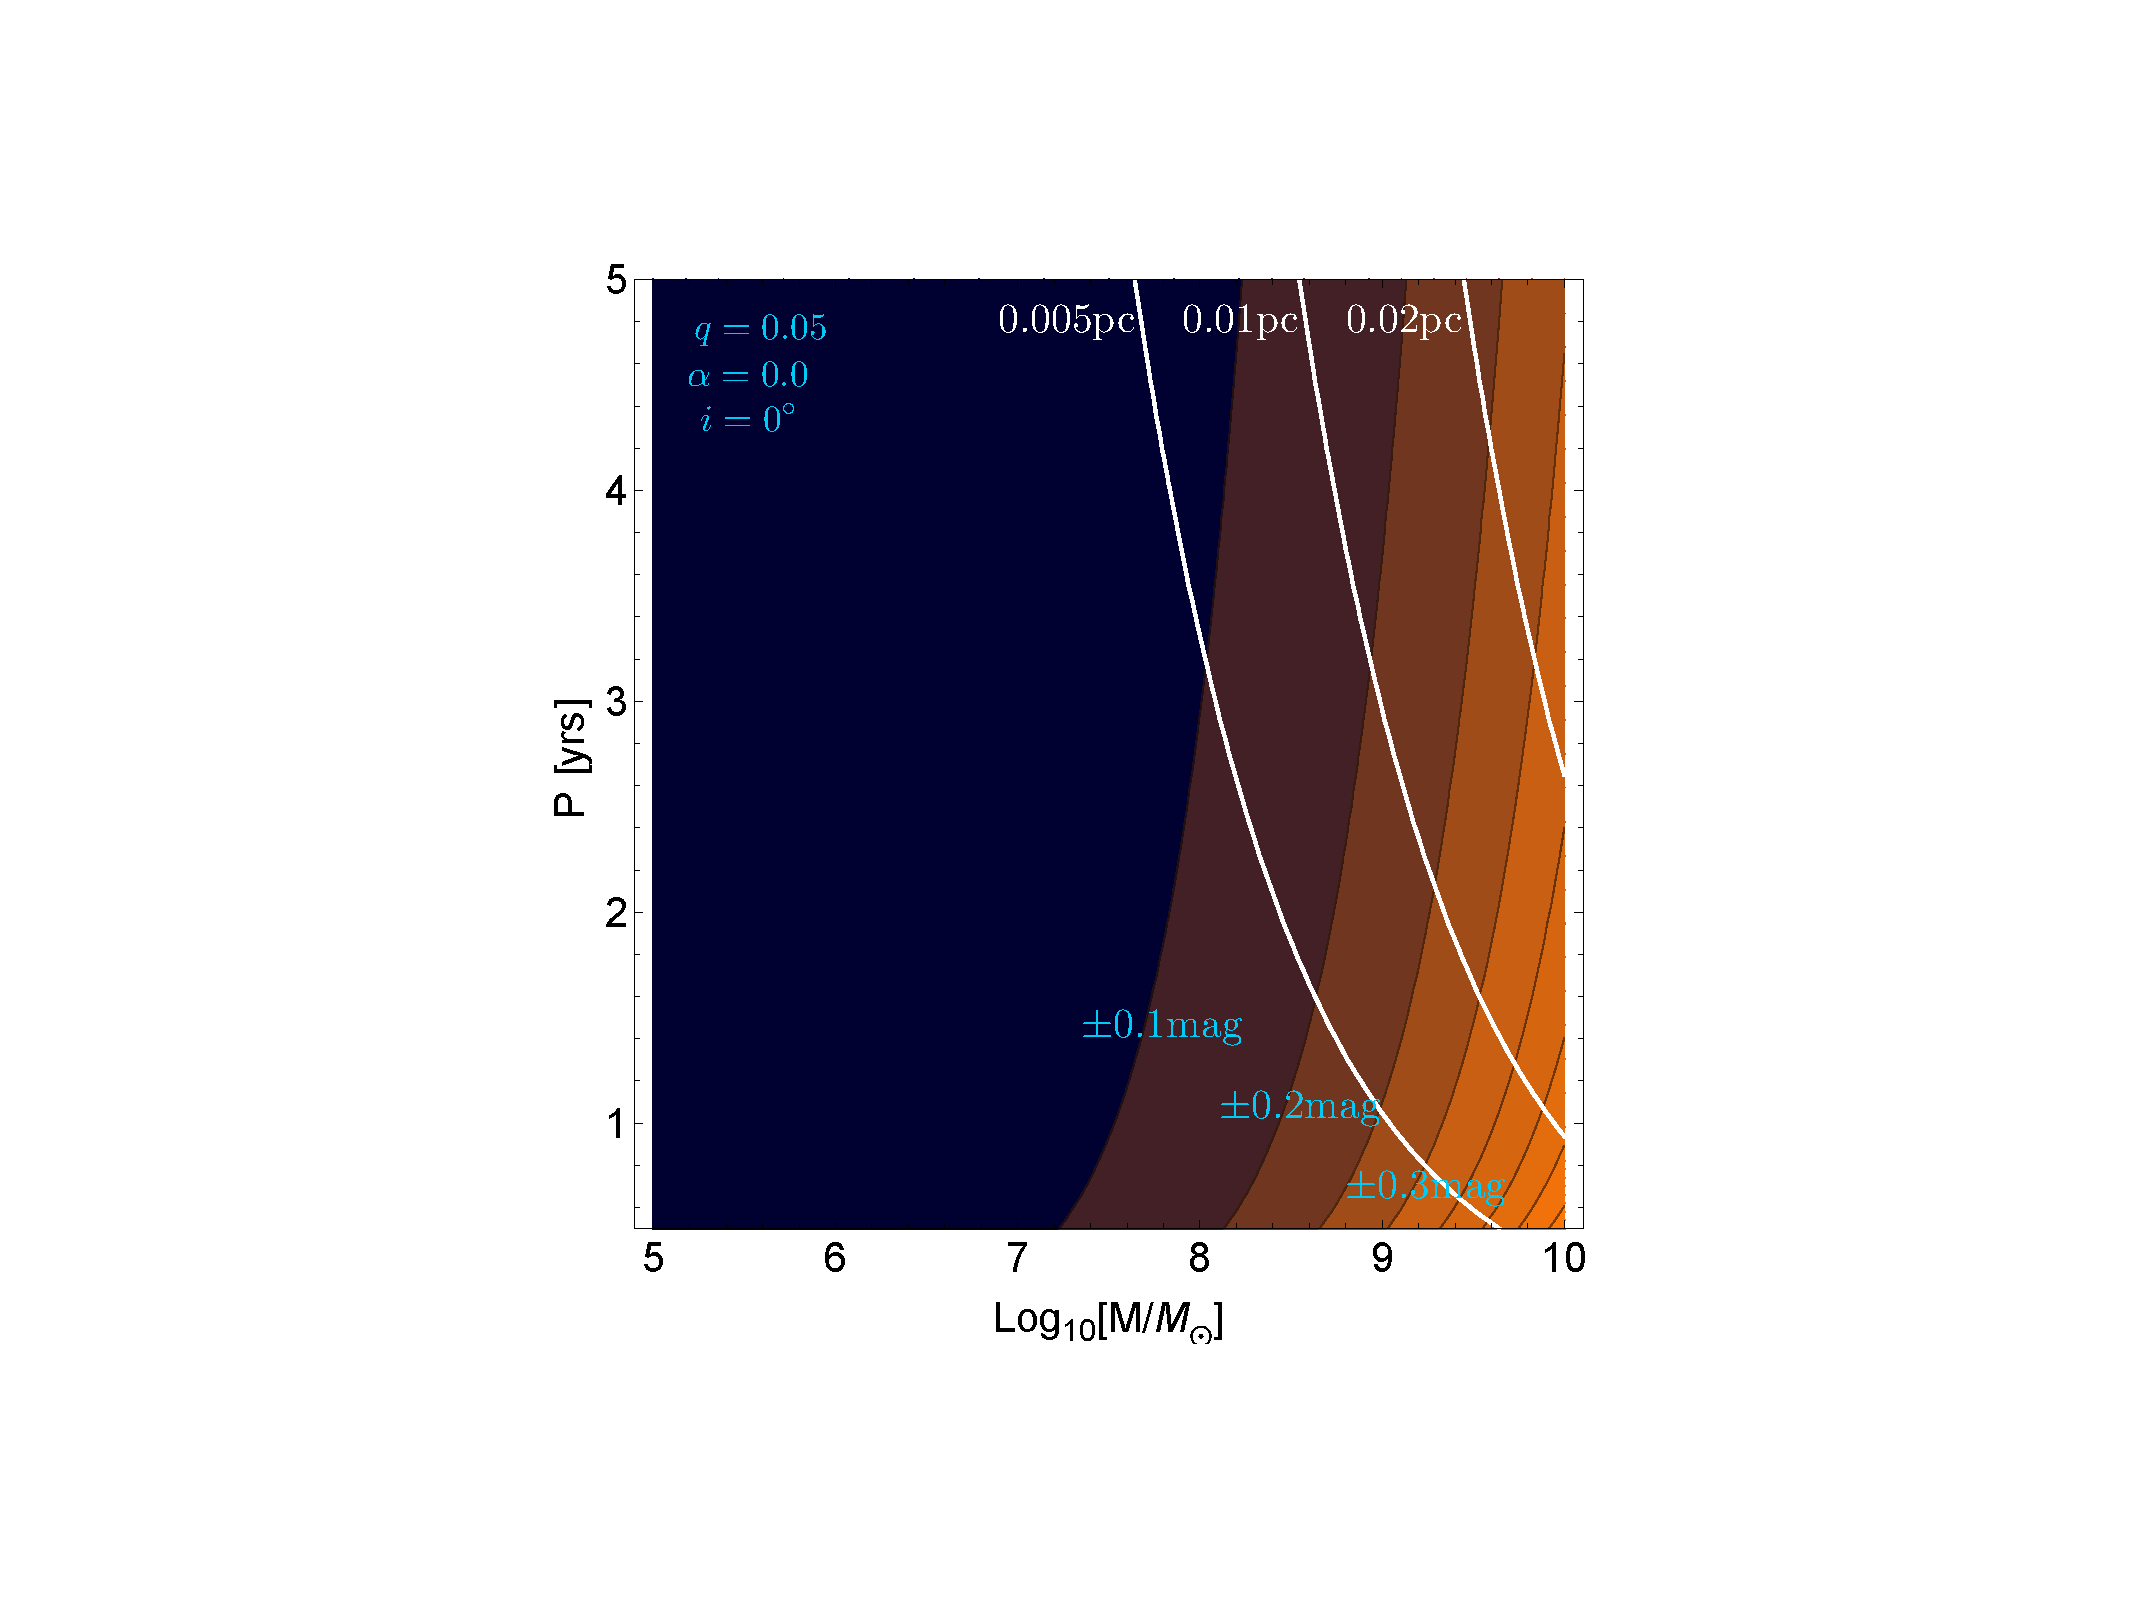
\includegraphics[scale=0.3]{figures/ch5/boosting_Pbin_M.pdf} \hspace{20pt} 
%
\end{array}$
\end{center}
\caption{Representative binary total masses and orbital periods for which boosting is an important cause of periodicity. White contours are different binary separations at the given orbital period and mass. Here we have assumed a mass ratio of $q=0.05$, an edge-on viewing of the binary, and a spectral index $\alpha=0.0$.}
\label{Fig:boostParams}
\end{figure}
%%%%%%%%%%%%%%%%%%%%%%%%%%%%%%%%%%%%%%%%%%%%%%%%


\subsection{System scales} 
Now that we have identified the properties of the
central illuminating source of UV and optical emission and the properties of
the surrounding dust, we determine some basic size scales of the system. The
most important size scales are the binary separation and the inner edge of the
dust distribution. The binary separation is given by the total binary mass $M$
and orbital period $P$
\begin{equation}
a = \left(\frac{P}{2 \pi} \sqrt{GM} \right)^{2/3}.
\end{equation}
The inner edge of the dusty torus is set by the onset of dust sublimation. For a source with luminosity $L = \epsilon L_{\rm{Edd}}(M)$, dust sublimates at radii
\begin{equation}
\Rin \lsim 0.9 \epsilon^{1/2}_{0.1} \left(\frac{M}{10^9 \Msun }\right)^{1/2}  \left(\frac{1800 K}{ T_{\rm{sub}} }\right)^{2.6} \rm{pc},
\label{Eq:Rd}
\end{equation}
where $\epsilon_{0.1} \equiv 0.1$ assumes that the total binary luminosity is
one tenth of the Eddington rate, and we assume that the inner, hottest region
of the dust torus is composed of graphites which sublimate at temperature
$T_{\rm{sub}} \sim 1800 K$ \citep{MorTrakhtenbrot:2011, MorNetzer:2012}. $R_d$
is the inner edge of the dusty torus, which we treat as a free parameter in
our model but interpret in the context of Eq. (\ref{Eq:Rd}). We set the out
edge to where the optical depth to UV photons reaches unity.

%but we keep in mind that IR imaging finds IR radiation to come from a region of order the size of the inner edge of the dust region \citep[see][and references within]{Elitzur:2006}.


%It is also important to determine the optical depth of the source radiation to the dust and also optical depth of the emitted IR emission. The former determines the dust temperature throughout the dust distribution, the latter determines how we calculate the observed IR flux. 

Assuming a uniform dust number density $n_d$, the optical depth of the dust to
radiation is approximately
\begin{eqnarray}
\tau_{\nu} &=& n_d \pi a^2_{\rm{eff}} Q_{\nu} R \nonumber \\
& =& 1 \left( \frac{n_d}{4 \times 10^{-10} \rm{cm}^{-3}} \right) \left( \frac{a_{\rm{eff}}}{0.16 \mu \rm{m}} \right)^2  \left( \frac{Q_{\nu}}{1} \right)  \left( \frac{R}{1 \rm{pc}} \right),
\end{eqnarray} 
where $a_{\rm{eff}}$ is the radius of a dust grain, $R$ is a typical size
scale of the dust region, and $Q_{\nu}$ is the frequency dependent
absorption/emission efficiency of the dust. As discussed below, we choose
$Q_{\nu}$ so that it decreases as $\nu^n$ for $\nu \leq 1 \mu$m. For IR
emission in the $3 \rightarrow 10 \mu$m wavelength range of the WISE band,
$\tau_{\rm{W}} \sim ((1/3)^k \rightarrow (1/10)^k) \tau_{\rm{UV}}$, where
$\tau_{\rm{W}}$ is the optical depth to WISE band IR radiation and
$\tau_{\rm{UV}}$ is the optical depth to high frequency radiation from the
central source. Because $\tau_{\rm{W}}$ and $\tau_{\rm{UV}}$ are only in
different regimes for very steep cutoffs in efficiency and for marginal
optical depths, and because we do not a-priori know the dust density (many
optically thin and optically thick models exist), we consider multiple
assumptions for the dust optical depth below.


%Then because $\tau_{\rm{W}}$ and $\tau_{\rm{UV}}$ are only in different regimes for very steep cutoffs in efficiency and for marginal optical depths, and because we do not a-priori know the dust density (many optically thin and optically thick models exist), we work in two limits:
%\begin{enumerate}
%\item \textit{Optically Thin:} Both high frequency source radiation and long frequency dust emission is optically thin to the dust and we integrate total emission from dust out to where $\tau_{\rm{UV}} \sim 1$.
%\item \textit{Optically Thick:} $\tau_{\rm{UV}} \sim \tau_{\rm{IR}} \gg 1$ and we only need to integrate emission from the inner edge of the dust distribution and remove emission which is blocked by intervening dust.
%\end{enumerate}



\section{Model Derivation}
\label{S:Derivation}
\subsection{Isotropic emission from a central source}
\label{S:FISOderivation}
The novel addition to dust reverberation modeling that we put forth in this
work is the addition of a time-dependent anisotropic central source. To
compare to the case of an isotropic source and to aid in the build up to the
anisotropic case which heats a surrounding, geometrically-thick dusty torus,
we first consider an isotropic, time-dependent central source of continuum
emission for increasingly complex dust geometries. Unless stated, we assume
for illustrative purposes that the dust is optically thick to the UV/optical
continuum source radiation and optically thin to the reprocessed dust
emission, in this way we can first explore the dependence on dust geometry.

\subsubsection{Spherical Dust Shell}

We first assume the source with bolometric luminosity $L^{\rm iso}(t)$ to be
surrounded by a infinitely thin sphere of dust with radius $\Rin$. To
illustrate the dependence of lR light curves on dust geometry, we assume for
this case that all of the source luminosity is absorbed by the shell of grains
and remitted without further absorption (that the dust is optically thick to
UV, but optically thin to IR emission emitted by grains). We adopt spherical
coordinates centered on the dust shell ($r,\theta,\phi$), with the observer
situated at coordinates $(r,  \theta, \phi) = (d, \pi/2, 0)$. The specific
flux at the dust shell is
\begin{equation}
F^{\rm iso}_{\nu} = \frac{L^{\rm iso}_{\nu}}{4 \pi R^2_d}.
\end{equation}
This flux of continuum radiation heats the surrounding dust. By assuming that
the dust is in radiative equilibrium with the heating source, and given an
efficiency of absorption/emission by the dust $Q_{\nu}$, we find the dust
temperature as a function of time by equating the power absorbed by a dust
grain to that radiated,
\begin{eqnarray}
\pi a^2_{\eff}\bar{Q}^{\rm src}_{\nu} F^{\rm iso}(t) = 4\pi a^2_{\rm eff} \int^{\infty}_{0}{Q_{\nu} \pi B_{\nu}\left[T_d(t)\right] \ d \nu } ,
\label{Eq:TdISO}
\end{eqnarray}
where $a_{\rm eff}$ is the effective grain radius and we assume that the same
$a_{\eff}$ describes the dust cross section for absorption as well as the
surface area for emission, $Q_{\nu}$ is the absorption/emission efficiency of
the dust, $\pi B_{\nu}$ is the blackbody flux from a uniformly emitting dust
grain at temperature $T^{\rm iso}_d$, and $\bar{Q}^{\rm src}_{\nu}$ denotes an
average over the source spectrum.

Radiation with wavelength $\lambda = c/\nu \lsim 2 \pi a_{\eff}$ will be
absorbed efficiently by grains while for longer wavelength radiation, grains
of the same size become transparent, that is dust of a given grain species is
optically thin to radiation below some cutoff frequency. Hence for the
absorption/emission efficiency we choose $Q_{\nu}=1$ for frequencies above a
cutoff $\nu_0 \sim c (2 \pi a_{\eff})^{-1}$ and a power law fall off in
efficiency for lower frequency (long wavelength) radiation, $Q_{\nu} \equiv
\rm{min}\left[ (\nu/\nu_0)^k, 1\right]$ where $k \geq 0$. We take fiducial
values of $k=1$ and $c/\nu_0 = 1\mu$m such that our effective grain size is
$a_{\eff} \sim 0.16 \mu$m,  consistent with the allowable range of hot
Graphite grain sizes near the sublimation radius \citep{LaorDraine:1993,
MorNetzer:2012}. Because the efficiency for absorption is unity for high
frequency radiation, above $\sim$ $1\mu$m, we take $\bar{Q}^{\rm src}_{\nu} =
1$ throughout. In this work we fix the dust grain size and the dust
absorption/emission efficiency, however, the above parameters can also be left
as free parameters in order to fit for dust properties.


The observed flux due to one dust grain at temperature T is
\begin{eqnarray}
F^{\rm{grain}}_{\nu} &=& 2 \pi \int^{\theta_c}_0{ Q_{\nu} B_{\nu}(T) \cos{\theta_s} \sin{\theta_s} d \theta_s} = \left(\frac{ a_{\rm{eff}} }{d}\right)^2 Q_{\nu} \pi B_{\nu}(T) \\ \nonumber  
\theta_c &=& \sin^{-1}\left( \frac{ a_{\rm{eff}}}{d}\right) .
\end{eqnarray}
where $\theta_s = \theta_c$ is the angle subtended on the sky by a dust grain
with radius $ a_{\rm{eff}}$ at a distance $d$ from the observer. Given the
grain number density, the time dependent dust temperature everywhere in the
shell (Eq. (\ref{Eq:TdISO})), and again assuming in this case that dust is
optically thin to its own emission, we compute the total observed flux from
heated dust grains
\begin{eqnarray}
\label{Eq:FnuSS}
 F^{\rm SS}_{\nu}(t) &=& \left(\frac{ a_{\rm{eff}} }{d}\right)^2 \int^{2 \pi}_{0}{\int^{\pi}_{0}{ \Sigma_d Q_{\nu}  \pi B_{\nu}\left[T_d(t_{\em})\right]  R^2_d \sin{\theta} \ d \theta d\phi }}   \\ \nonumber 
 %
t_{\em}& =& t - \frac{\Rin}{c} \left( 1 - \sin{\theta} \cos{\phi}\right)  
\end{eqnarray}
where $\Sigma_d$ is the dust shell surface number density. The most important
aspect of the above equation is that we have evaluated the temperature at the
time $t_{\em}$; if light leaving the front of the dust shell reaches an
observer at time $t$, then light emitted from the location ($\Rin$, $\theta$,
$\phi$) will reach the observer at time $t_{\em}$. By integrating over all
locations in the dust shell at time $t$, we take into account the finite light
travel time. Put another way, we evaluate the time changing dust temperature
at the retarded time. The left panel of Figure \ref{Fig:Schm} illustrates this
by drawing cross sections of the parabaloids of constant light travel time
(described by the equation for $t_{\em}$). Conceptually, Figure
\ref{Fig:Schm}, along with the definition of $t_{\em}$, tells us that dust
emission at time $t$ is comprised of dust emission spanning a time interval of
$2 \Rin /c$ in the frame of the central emitting source. The lesson being that
the reprocessed dust emission will not necessarily be a phase shifted replica
of the continuum emission.


The total observed flux at an instrument with bandpass function $W(\nu)$ is
 \begin{equation}
F_{W} = \int^{\infty}_{0}{  W(\nu) F_{\nu} d \nu  } \sim \int^{\nu_{\rm max}}_{\nu_{\rm min}}{ F_{\nu} d \nu}
\label{Eq:FISO}
 \end{equation}

where we have assumed that $W(\nu)$ is a top hat function with frequency
limits $\nu_{\rm min}$ and $\nu_{\rm max}$.


%We now expand upon this basic model with more complex dust geometry and source flux.

%To apply this simple dust reverberation model to the case of MBHBs in galactic nuclei we now change the form of the central luminosity source and allow a more realistic dust geometry.
 %%%%%%%%%%%%%%%%%%%%%%%%%%%%%%%%%%%%%%%%%%%%%%%%
%%% FIGURE: Light Travel Geometry %%%
%%%%%%%%%%%%%%%%%%%%%%%%%%%%%%%%%%%%%%%%%%%%%%%%
\begin{figure}
\begin{center}$
\begin{array}{c c }
%
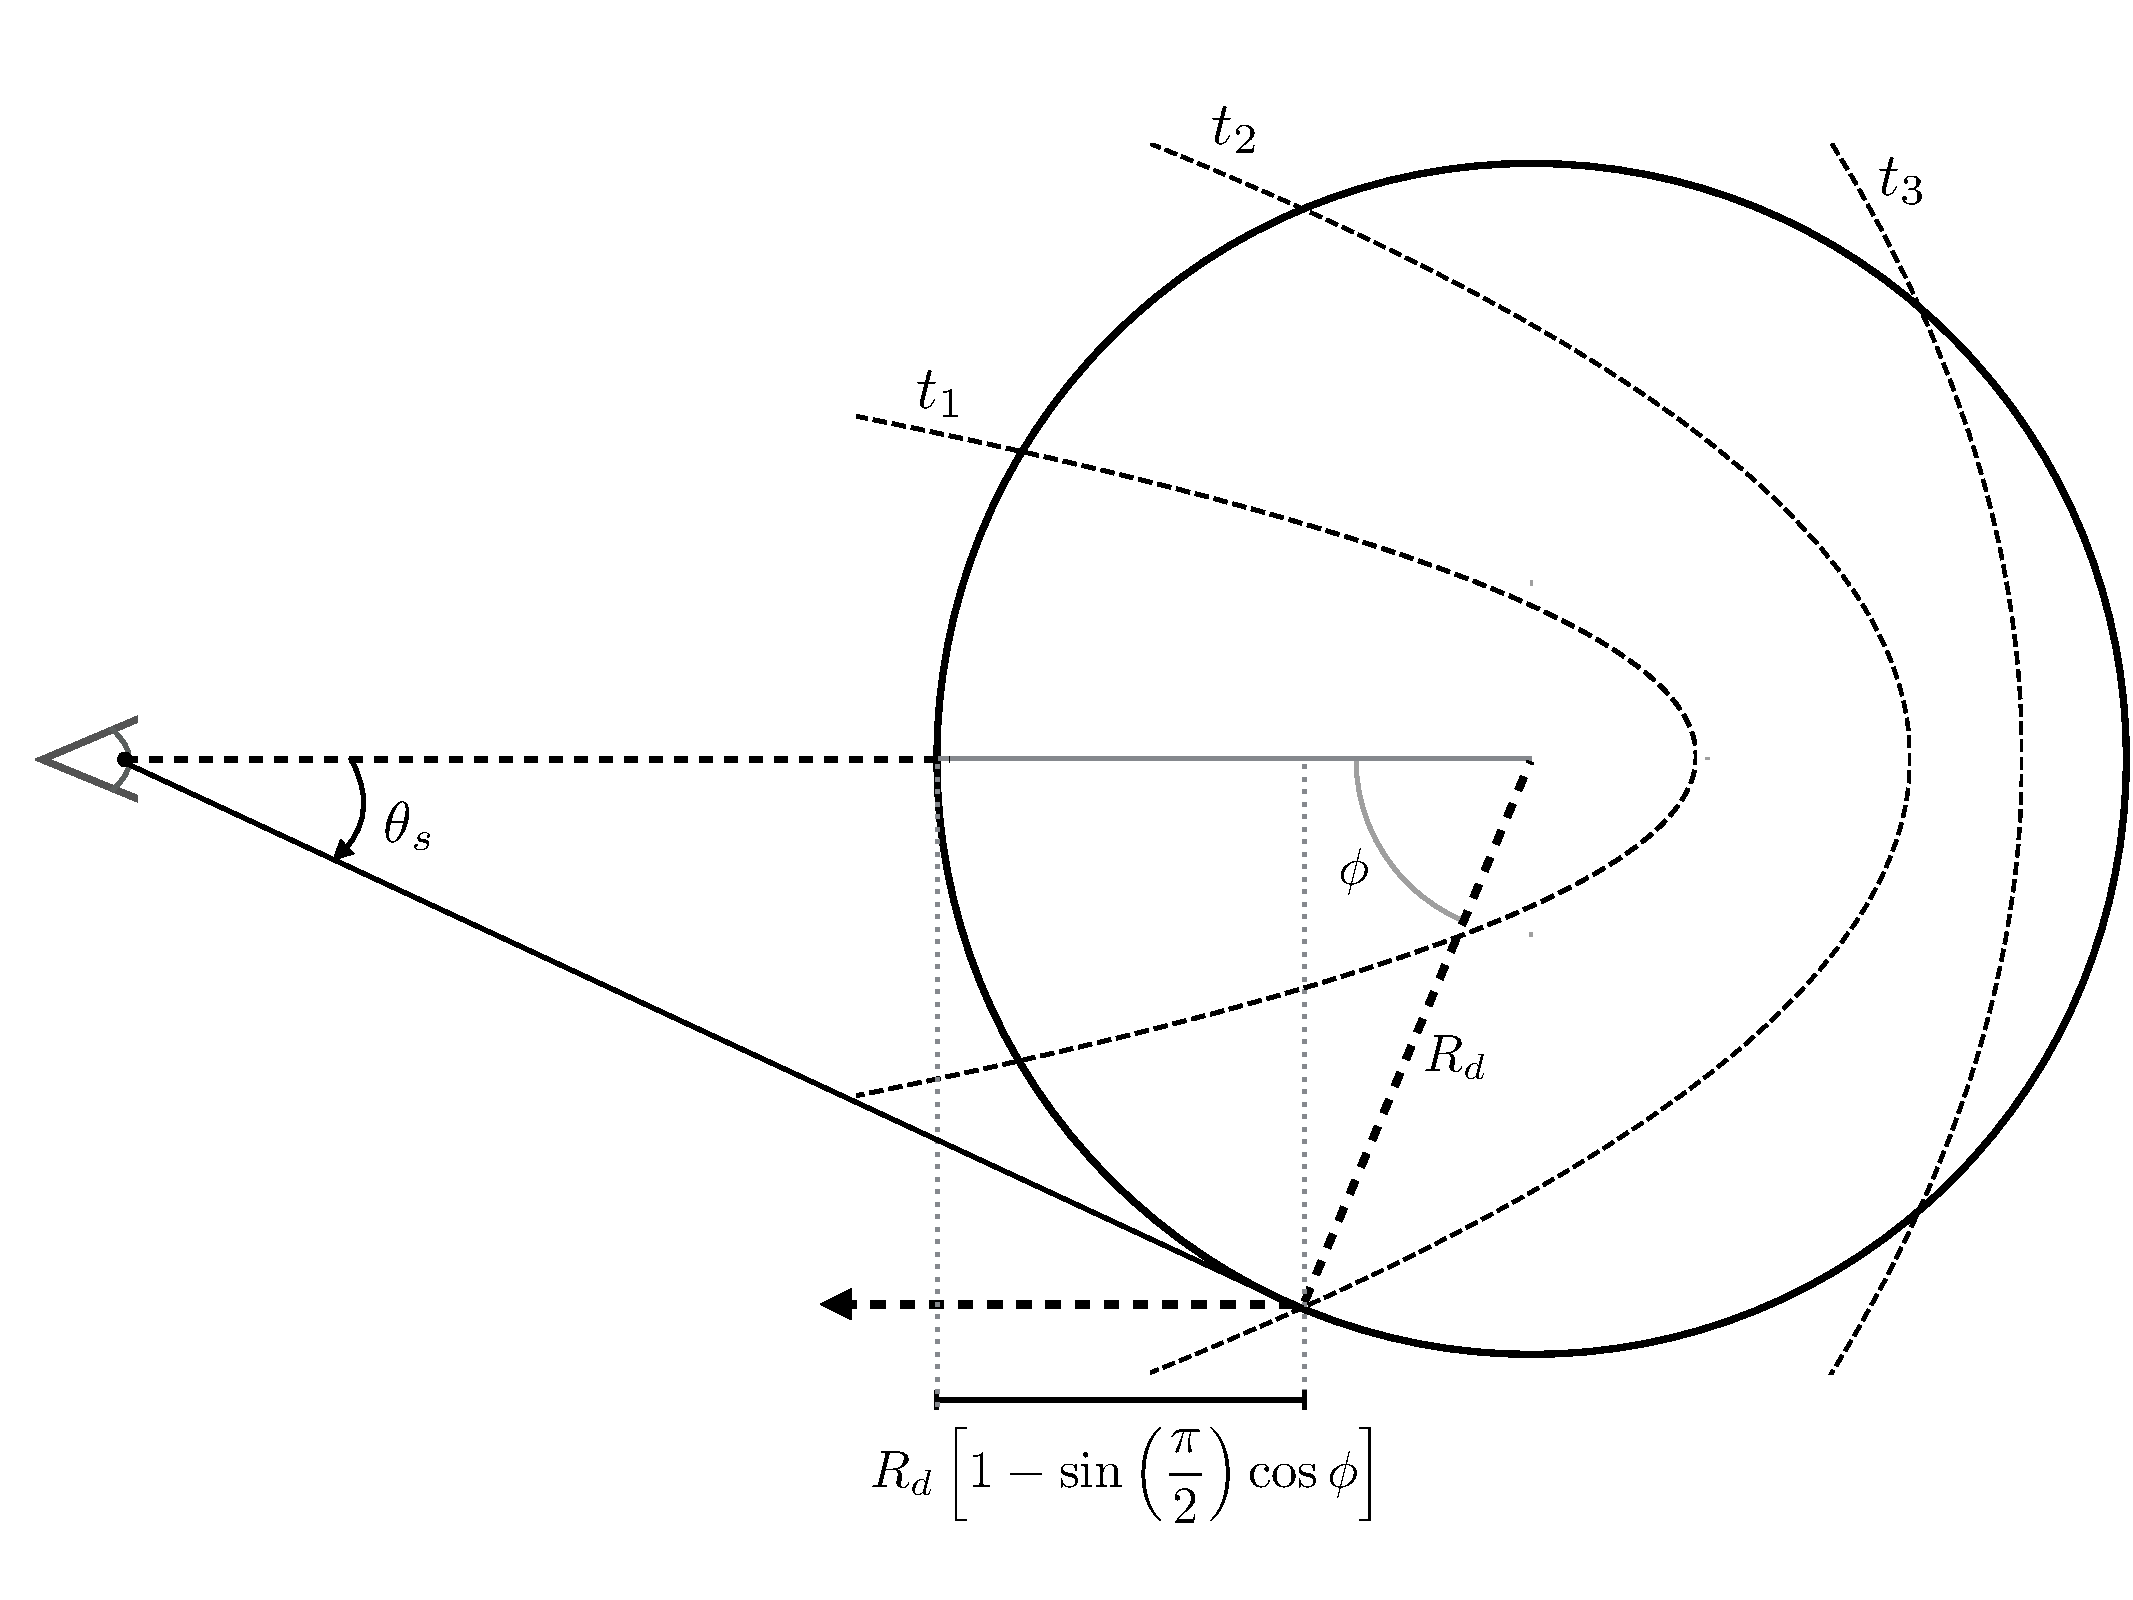
\includegraphics[scale=0.22]{figures/ch5/tem_schematic} \hspace{20pt} & 
 \includegraphics[scale=0.22]{figures/ch5/Torus_Schematic} 
%
\end{array}$
\end{center}
\caption{Left: light travel time geometry. Right: angles present in Torus geometry.}
\label{Fig:Schm}
\end{figure}
%%%%%%%%%%%%%%%%%%%%%%%%%%%%%%%%%%%%%%%%%%%%%%%%



%%%% COME BACK TO THE RING!
% %%%%%%%
% %%%%%%%
\subsubsection{Dust Ring}
The spherical shell dust model has a single geometric parameter, the radius of
the shell $R_d$. We now introduce a second parameter by considering a ring of
dust at inclination $J$ to the observer's line of sight. The reverberated
emission form a ring of dust with radius $R_d$ at an angle $J$ to the observer
plane (x -y plane) is found from integrating Eq. (\ref{Eq:FnuSS}) over the
position of the ring,
\begin{eqnarray}
\label{Eq:FnuRing}
 F^{\rm Ring}_{\nu}(t) &=& \left(\frac{ a_{\rm{eff}} }{d}\right)^2 \int^{2 \pi}_{0}{{ l_d Q_{\nu}  \pi B_{\nu}\left[T_d(t_{\em})\right]  R_d \sin{\theta_R(\phi)} \  d\phi }}   \\ \nonumber 
 %
%\theta_R(\phi)& =& \rm{arctan2}\left[ \rm{sign}(\cos{\phi}) \cos{J} \sqrt{1 +  \left( \frac{\tan{\phi}}{\cos{J}} \right)^2}, - \sin{J} \right] - \frac{\pi}{2} \left[ \rm{sign}(\cos{\phi}) - 1\right]
\theta_R(\phi)& =& \tan^{-1}\left[ R^2_d \left(\cos^2{J} + \sin^2{\phi'}\sin^2{J}\right), R_d \cos{\phi'} \sin{J} \right] \nonumber \\
&&\sin{\theta_R} \sin{\phi'} = \sin{\phi}
\end{eqnarray}
where $l_d$ is the linear dust number density of the ring taken to be $l_d =
1/{2a}$ in the limit that the ring is made entirely of grains, which is
sufficient for the illustrative purposes of this model.


%%%%%%%
%%%%%%%
\subsubsection{Torus Shell}
\paragraph{Optically thin}
We next remove portions of the sphere to consider a torus with infinitely
small radial extent. This introduces a third dust geometry parameter
$\theta_T$ which gives the opening angle of the torus such that the previous
case of a dust ring is the limit in which $\theta_T \rightarrow \pi/2$. These
angles and the binary inclination angle are drawn schematically (for a torus
with finite radial extent) in the right panel of Figure \ref{Fig:Schm}. For
the torus model we simply set the temperature found in Eq. (\ref{Eq:TdISO}) to
zero for
\begin{eqnarray}
\theta'(J) < \theta_T \quad \rm{or} \quad \theta'(J) > \pi - \theta_T
\end{eqnarray}
where $\theta'(J)$ is the polar coordinate in a coordinate system rotated
around the y axis by angle $J$.




%%%%%%%
%%%%%%%
\paragraph{Optically thick}
To capture the effects of obscuration by the torus on the observed IR
continuum, we consider a case where the dust is optically thick to the IR dust
emission \emph{in addition to} the UV/optical source emission.

Then instead of integrating over all IR emission from the dust shell, as in
the previous case, we block emission which intersects dust along the line of
sight. In practice we do not include emission which emanates from the near
side of the dust distribution $(x>0)$ and we do not include emission emanating
from the far side of the dust distribution ($x<0$), from a point $(x, y, z)
\ni x<0$, if
\begin{eqnarray}
\theta'(J) \geq \theta_T \quad \rm{and} \quad \theta'(J) \leq \pi - \theta_T
\end{eqnarray}

Note that for torus inclination angles $\pm(\pi/2 - \theta_T) \leq J \leq
\pm(\pi/2 + \theta_T)$, the observer's view of the central source is
unobscured (see the right panel of Figure \ref{Fig:Schm}). The observed flux
is computed identically to Eq. (\ref{Eq:FnuSS}).



%%%%%%%
%%%%%%%
\subsubsection{Torus with Finite Extent}
\label{S:ThickTor}
Our final dust model introduces a two more dust parameters describing the radial dust density distribution. We assume the dust is optically thin
to UV/optical out to some radius $R_{\tau=1}$ and optically thin to IR
dust emission.  To give the dust shell a finite thickness we provide the dust
number density as a function of radius
\begin{eqnarray}
n_d(r)
&=& 
\left\{
        \begin{array}{l l}
              &n_0 \left(\frac{\Rin}{r}\right)^{p}  \quad  \Rin < r < \Rout    \qquad p>0 \\
              &0   \qquad \qquad \quad \ \  \mbox{else} % r < \Rin  \ \bigcup  \  r> \Rout .
        \end{array}
\right.
\label{Eq:nd}
\end{eqnarray}
As light from the central source illuminates the dust, source photons will be
absorbed with efficiency $Q_{\nu}$, as before, heating the dust. Absorption
also attenuates the flux reaching further into the dust structure. The
radiative transfer equation for the specific intensity along a ray is
\begin{eqnarray}
\frac{d I_{\nu}}{dr} &=& -\kappa_{\nu}I_{\nu}  \nonumber \\
 &=& -  n_d(r) \pi a^2_{\rm eff} {Q}_{\nu} I_{\nu},
\end{eqnarray}
where $\kappa_{\nu} = n \sigma_{\nu}$ is the absorption coefficient of the dust. The solution for the specific intensity in this case is
\begin{eqnarray}
I_{\nu}(r) &=& I_{\nu}(\Rin)  \rm{e}^{ -\tau_{\nu}(r)} \\ \nonumber
\tau(r)  &=&  
\left\{
        \begin{array}{ll}
              & \frac{ n_0 \pi a^2_{\rm eff} \bar{Q}_{\nu}}{p - 1} \Rin \left[ 1 - \left( \frac{\Rin}{r}\right)^{p-1} \right]   \quad \Rin < r < \Rout    \\
              &0   \qquad \qquad \qquad \qquad \qquad  \qquad \quad  \mbox{else}.% r < \Rin  \ \bigcup  \  r> \Rout .
        \end{array}
\right.
\label{Eq:tauIn}
\end{eqnarray}
where we have integrated over frequency of the central source emission. The
dust is optically thin to the source emission out to
\begin{equation}
\label{Eq:Rtau1}
R_{\tau=1} = \frac{R_d} {\left[ 1 - \frac{p-1}{n_0 a^2_{\rm eff} \bar{Q}_{\nu} \pi }  \right]^{\frac{1}{p-1}}}.
\end{equation}
%
The dust temperature is now given by
\begin{eqnarray}
\bar{Q}^{\rm src}_{\nu} F^{\rm iso}(t)  \rm{e}^{ -\tau(r)} = 4 \int^{\infty}_{0}{Q_{\nu} \pi B_{\nu}\left[T_d(t, r)\right] \ d \nu } ,
\label{Eq:TdISO2}
\end{eqnarray}
and the IR flux is given by
\begin{eqnarray}
\label{Eq:Fnu_Thick}
 F^{\rm Torus}_{\nu}(t) &=& \left(\frac{ a_{\rm{eff}} }{d}\right)^2 \int^{R_{\tau=1}}_{R_d}{ \int^{2 \pi}_{0}{\int^{\pi}_{0}{ n_d Q_{\nu}  \pi B_{\nu}\left[T_d(t_{\em}, r)\right]  R^2_d \sin{\theta} \ d \theta d\phi  dr}} }  \\ \nonumber 
 %
t_{\em}& =& t - \frac{r}{c} \left( 1 - \sin{\theta} \cos{\phi}\right)  
\end{eqnarray}








%%%%%%% 
\subsection{Non-isotropic, Doppler boosted emission - the lighthouse} 
%%%%%%% 
To include the effects of Doppler beaming in the IR light
curve we only need to change the source flux. We assume that dust surrounds a
binary with total mass $M$ and separation $a$. Due to relativistic Doppler
boosting of a steadily emitting source attached to the secondary, the specific
flux received in the frame of the stationary dust shell differs from the
specific flux in the rest frame of the secondary BH as dictated by Eq.
(\ref{Eq:Dop1}). Assuming a rest frame flux $F^0_{\nu} \propto
\nu^{\alpha_{\nu}}$, the flux at the location of the dust shell is,
\begin{eqnarray}
F_{\nu}(t, \Rin, \theta, \phi) &=& \left[D(t, \theta, \phi)\right]^{3-\alpha_{\nu}} F^0_{\nu}(\Rin)  \nonumber \\
&=&  \left[D(t, \theta, \phi)\right]^{3-\alpha_{\nu}} \frac{L^0_{\nu}}{4 \pi r^2_2}  \\ \nonumber
D(t, \theta, \phi) &\equiv& \left[ \gamma \left(1 - \frac{v_{||}}{c} \right) \right]^{-1},
\label{Eq:DopFlux}
\end{eqnarray}
where $L^0_{\nu}$ is the rest frame, specific luminosity of the source,
$\gamma = \left[ 1 - (v_s/c)^2 \right]^{-1/2}$ is the Lorentz factor of the
secondary which orbits at speed $v_s = (1+q)^{-1}\sqrt{GM/a}$, $I$ is the
inclination angle of the binary's orbit to the line of sight, $\Omega$ is the
angular frequency of the binary and we assume throughout that the binary is on
a circular orbit. We continue to use the spherical coordinates as above with
($r,\theta, \phi$) centered on the binary center of mass and with the observer
situated at ($d,\pi/2$,0). We have approximated the distance from the
secondary to the dust shell as $\Rin$ (see Eq. \ref{Eq:aORd} below).

The line of sight velocity $v_{||}$ in the Doppler factor $D$ is the line of
sight speed of the secondary BH as  observed by a dust grain at position
$\mathbf{\hat{r}}_{\rm{dust}}$ in the dust shell. Written in terms of
barycentric coordinates $(r,\theta, \phi)$,
\begin{eqnarray}
\frac{v_{||}}{c} &=& \frac{\mathbf{v_{s}} \cdot \mathbf{\hat{r}}_{\rm{dust}} }{c}\\ \nonumber 
& = & \beta  \left[ \cos{I} \cos{(\phi_0+\Omega t)} \sin{\theta}\cos{\phi} - \sin{(\phi_0+\Omega t)} \sin{\theta}\sin{\phi} - \sin{I} \cos{(\phi_0+\Omega t)} \cos{\theta}  \right],
\label{Eq:vlos}
\end{eqnarray}
where $\phi_0$ is the $\phi$ coordinate of the secondary at $t=0$ and we have
parameterized the secondary orbital velocity as $\beta \equiv a (1+q)^{-1}
\Omega$ which depends on the binary mass ratio $q$, total mass $M$, and period
$P$ through the binary orbital frequency $\Omega$ and separation $a$.



Just as for the isotropically emitting source we can determine the temperature
of each patch of the dust shell, at each moment in time, from requiring that
the dust absorbs the incident radiation with some frequency dependent
efficiency $Q_{\nu}$ and comes to thermal equilibrium with the incident
radiation. The difference here is that the incident flux and resulting dust
temperature are now spatially varying across the sphere. The analogue of Eq.
(\ref{Eq:TdISO2}) becomes
\begin{equation}
\label{Eq:TdDop1}
\bar{Q}_{\nu} \int^{\infty}_{0}{F_{\nu}(t, \theta, \phi)  \ d \nu } =   4 \int^{\infty}_{0}{Q_{\nu} \pi B_{\nu}\left[T_d(t,\theta, \phi)\right] \ d\nu}.
\end{equation}
We approximate the LHS of the above equation as
\begin{equation}
\label{Eq:TdDop}
\left[D(t, \theta, \phi)\right]^{3-\bar{\alpha}} \frac{L^0}{4 \pi R^2_d}  =   4 \int^{\infty}_{0}{Q_{\nu} \pi B_{\nu}\left[T_d(t,\theta, \phi)\right] \ d\nu}. 
\end{equation}
where $L^0$ is the bolometric source luminosity and we have approximated the
frequency dependent source spectra slope $\alpha_{\nu}$ by an average
$\bar{\alpha}$ over source frequency. This solution for the dust temperature
can be used in either of the solutions for $F_{\nu}$ derived for an isotropic
source in \S \ref{S:FISOderivation}.



\section{Parameter Dependencies}
\label{S:PDs}

We now identify the important model parameters and their effect on the IR
light curves. The main parameters and their fiducial values are listed in
Table \ref{Table:params}.
%
\begin{table}
\begin{center}
\begin{tabular}{ c | c | c | c}
        Parameter         & Meaning     & Fiducial Value   &   Notes \\
                   \hline 
                  Binary Parameters &  & \\
                  \hline	
$L_0$				 & Bolometric source luminosity            & $6.78\times10^{46}$  erg s$^{-1}$	  & PG 1302 value\\
$\bar{\alpha}$                     &Source averaged spectral index     &  0.0  & \\
%$M$                                     & Total Mass        & $10^{9.1} \rightarrow 10^{9.4} \Msun $      \\
$\Omega$                          & Orbital frequency     			 & $2 \pi c/R_d $     & \\
%$q$                                       & Mass ratio           & $\lsim 0.1$    \\
$\beta$				 & Boost velocity$/c$  			& $0.068$   & Inferred from binary mass, period, and mass ratio. \\
$I$                                      & Inclination           				&  $0.0$  & $0^{\circ}$ is edge-on \\%Inferred from $\beta$ and variability magnitude   \\
                   \hline 	
                  Dust Parameters &  & \\
                  \hline	
$\Rin$               &  Inner edge of dust       								& $0.9 \sqrt{\epsilon/0.1}$ pc		& Sublimation radius for Graphites\\
{$n_0$}            &  Density normalization 								& $(p-1) (\pi a^2_{\eff} \Rin)^{-1}$	&		\\
{$p$}                &  Density exponent       								& 2.0 						&	$n_d(r) = n_0 \left( \Rin/r \right)^{p}$	\\
{$J$}                &  Torus inclination          								& $\pi/2$						&	0 obstructed; $\pi/2$ un-obstructed	\\
{$\theta_T$}     &  Torus opening angle   								  & $\pi/4$						&	\\
%$\Rout$            &  Outer edge of dust      								& $10\Rout$ 					& weak dependence for $p>0$		\\
$k$		        &  Absorption/emission efficiency exponent       				& 1 							&	\\
$\nu_0$		& Efficiency cutoff frequency							&    $c/(2 \pi a_{\rm{eff}})$			& $Q_{\nu} = \rm{min}\left[ \left( \nu/ \nu_0 \right)^{k}, 1\right]$	\\
$a_{\rm{eff}}$	&  Grain size         	       								&  $0.16$ $\mu$m		       		&  Set by $\nu_0$		
 \end{tabular}
\caption{Parameters of the model and their fiducial values chosen for this study.}
\label{Table:params}
\end{center}
\end{table}
%
Figures \ref{Fig:Sph} through \ref{Fig:TorThick} explore the effect of varying these parameters and compare the use of an isotropically varying source to the Doppler boost varying source. In each figure we compute the UV/optical light curve for reference as a dashed line, and we compute the reprocessed IR light curves integrating over a large frequency range, from 30 GHz  (1m) to $3\times10^{16}$ Hz (10 nm) so that effects due to moving in and out of a particular waveband are muted. 



\subsection{Sphere}

The only dust parameter is $\Rin$, the radius of the dust inner edge. This
sets the temperature, and IR frequency of the emitted dust. For the Doppler
boosted central source, the binary inclination is also relevant. 

The top row of Figure \ref{Fig:Sph} shows IR light curves for different values
of the dust sphere radius and for the isotropic case (left) and the Doppler
boost case (right). For identical dust distributions, the IR light curves
differ in amplitude and phase, but are at roughly the same average magnitude.
The most noticeable difference is the red curve in the top row, for a dust
shell with radius such that the dust shell light crossing time is the same as
the period of source flux variations. In this case, light travel time delays
cause the light arriving at the observer from the front of the dust shell to
be completely out of phase with dust arriving at the observer from the back of
the shell. Hence the variation cancels in time for this specific geometry. The bottom left panel illustrates this further by plotting light curves from the same dust distributions as the top left panel, but with a 10 times faster source periodicity, removing the de-phasing effect present in the top panel.
%This does not occur in the Doppler case.



The bottom right panel highlights the importance of binary inclination in the
Doppler model. The inclination of the binary to the line of sight $\mathbf{I}$
sets the amplitude of modulation of both the prompt (UV and optical) and
reprocessed (IR) emission. The effect of the prompt emission is apparent from
the dependence of the Doppler factor in equation \ref{Eq:DopFlux} on the line
of sight orbital velocity $v_{||}$. The dependence of reprocessed IR emission
on the binary inclination is elucidated in the case of an optically thin
spherical dust distribution. 

The bottom right panel of Figure \ref{Fig:Sph}
shows that in this case, no variability is exhibited in the reprocessed
emission if the binary is face on. This is because if the light travel time
was not taken into account, integrating emission over the entire sphere would
yield no variability (not true for the isotropic case). Variability comes from
changes in the dust temperature distribution in time between the back and
front hemispheres of the shell. Because we are seeing front and back parts of
the dust at different times, we do not see the entire symmetric temperature
distribution at once, and the part that we see changes in time as different
components of the Doppler boosted emission heat the dust differently between
front and back hemispheres. This is why the top left panel of Figure
\ref{Fig:Sph} still shows variability in the red line for which the isotropic
case shows none. At face on inclination, the integrated dust temperature
distribution does not change between front and back hemispheres of the dust
sphere and so the total integrated flux is invariable. 

From this we may also conclude that the variability amplitude will increase
when obscuring material blocks some of the sphere, or when the dust is in a
torus geometry.





%%%%%%%%%%%%%%%%%%%%%%%%%%%%%%%%%%%%%%%%%%%%%%%%
%%% FIGURE: Sphere 1 ISO vs Dop%%%
%%%%%%%%%%%%%%%%%%%%%%%%%%%%%%%%%%%%%%%%%%%%%%%%
\begin{figure}
\begin{center}$
\begin{array}{c c}
%FISO and DOP  vary Rin
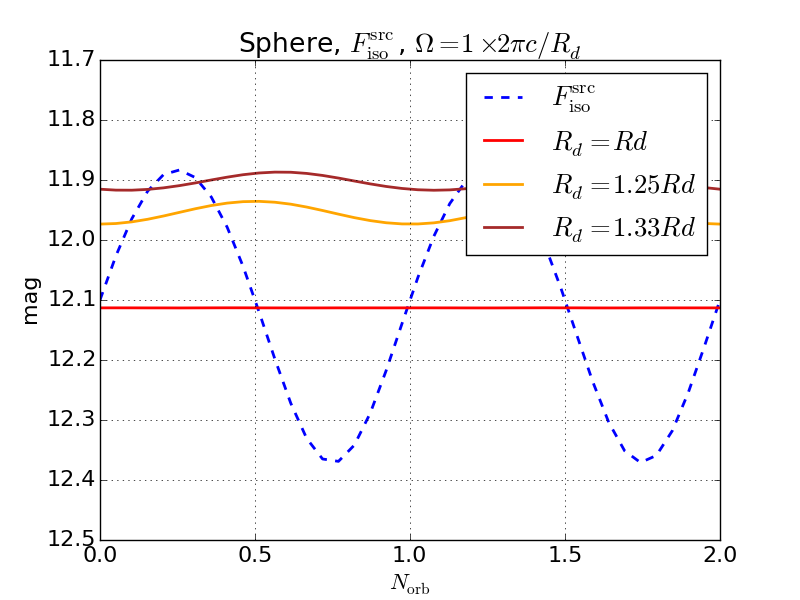
\includegraphics[scale=0.27]{figures/ch5/Sphere/FISO_Sphere_nrm1p50867_Om1_VaryRin_numin1e-05_numx100} & 
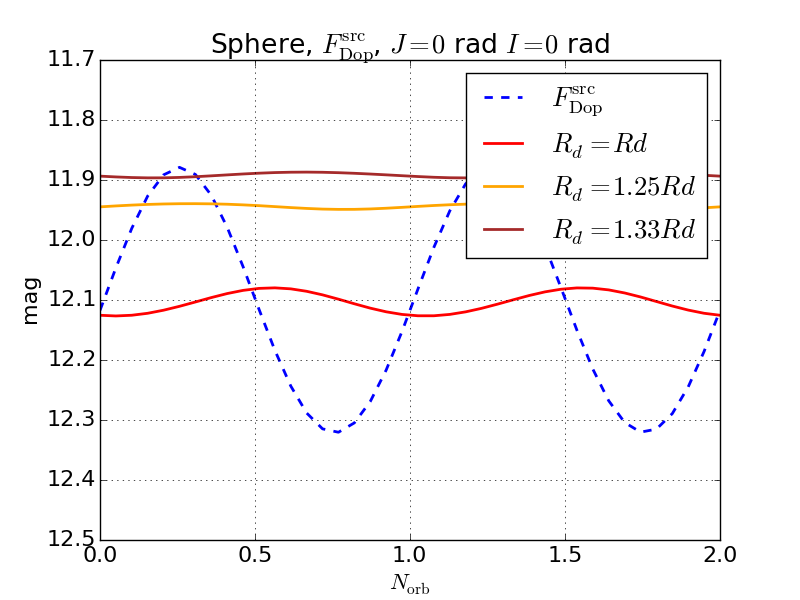
\includegraphics[scale=0.27]{figures/ch5/Sphere/FDop_Sphere_nrm1p50007__J0_Inc0_VaryRin_numin1e-05_numx100} \\
%
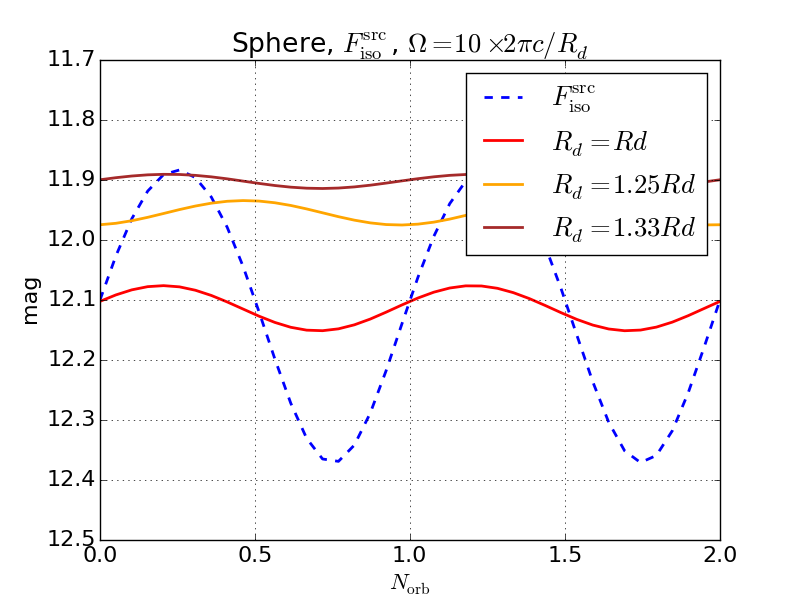
\includegraphics[scale=0.27]{figures/ch5/Sphere/FISO_Sphere_nrm1p50862_Om10_VaryRin_numin1e-05_numx100} & 
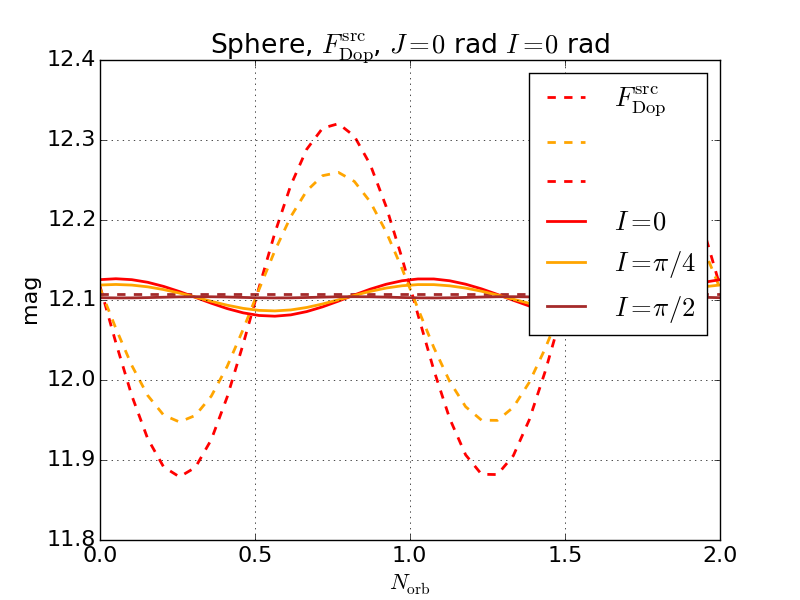
\includegraphics[scale=0.27]{figures/ch5/Sphere/FDop_Sphere_nrm1p50007_Rde2p73218e+18_VaryInc_numin1e-05_numx100} 
\end{array}$
\end{center}
\caption{Spherical dust shell model. The top row shows the difference in the isotropic and Doppler boost cases and also the dependence on the inner dust radius. The bottom row shows the dependence on binary inclination angle for the Doppler boosted source and the source period dependence for the isotropic source. When the period of source variation equals the light travel time from source to dust shell, the IR variation is washed out.}
\label{Fig:Sph}
\end{figure}
%%%%%%%%%%%%%%%%%%%%%%%%%%%%%%%%%%%%%%%%%%%%%%%%
















\subsection{Ring}
This case is left for future wrk.

% %%%%%%%%%%%%%%%%%%%%%%%%%%%%%%%%%%%%%%%%%%%%%%%%
% %%% FIGURE: Ring ISO vs Dop%%%
% %%%%%%%%%%%%%%%%%%%%%%%%%%%%%%%%%%%%%%%%%%%%%%%%
% \begin{figure}
% \begin{center}$
% \begin{array}{c c c}
% %
% 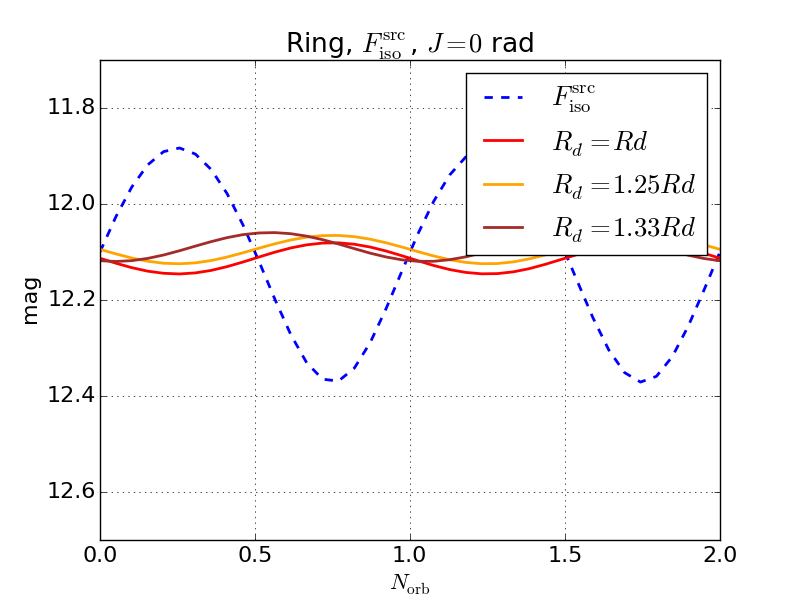
\includegraphics[scale=0.27]{figures/Ring/FISO_Ring_nrm-9p32812__J0_VaryRin_numin1e-05_numx100} & 
% 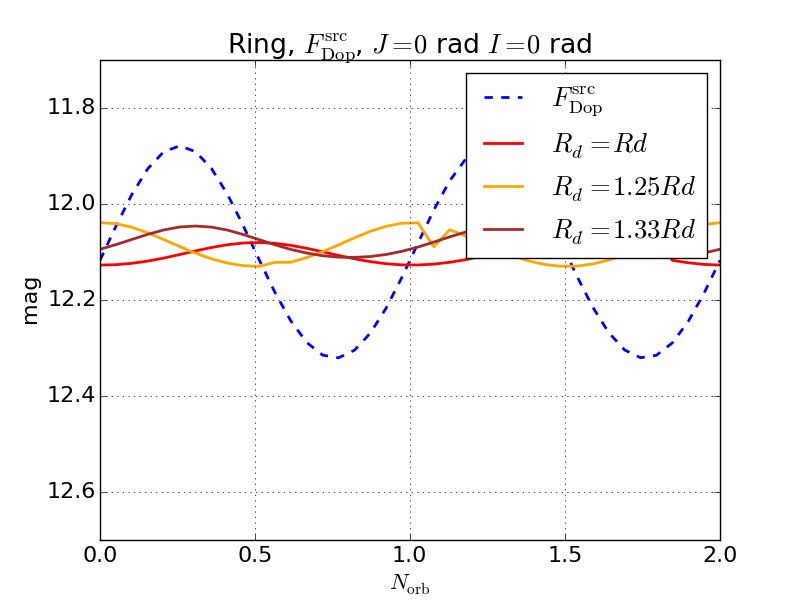
\includegraphics[scale=0.27]{figures/Ring/FDop_Ring_nrm-9p32931__J0_Inc0_VaryRin_numin1e-05_numx100}  &
% 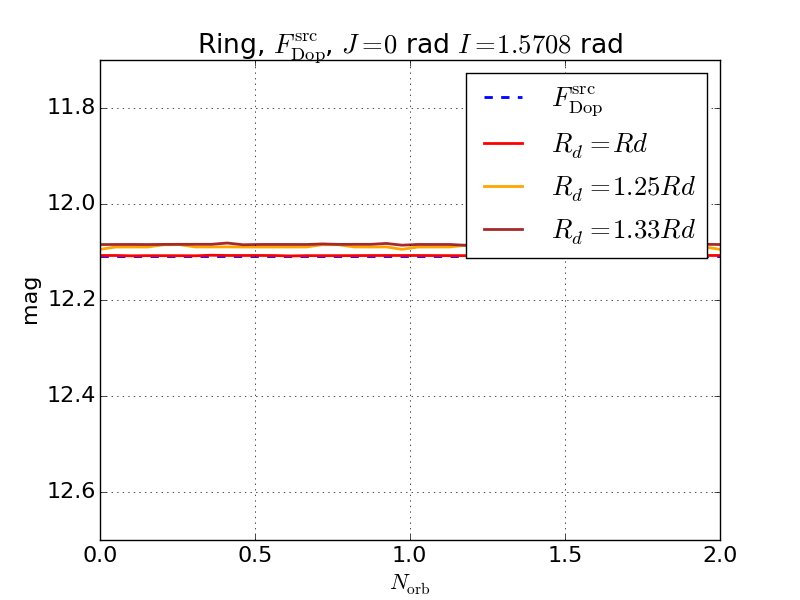
\includegraphics[scale=0.27]{figures/Ring/FDop_Ring_nrm-9p33301__J0_Inc1p5708_VaryRin_numin1e-05_numx100}\\
% %
% 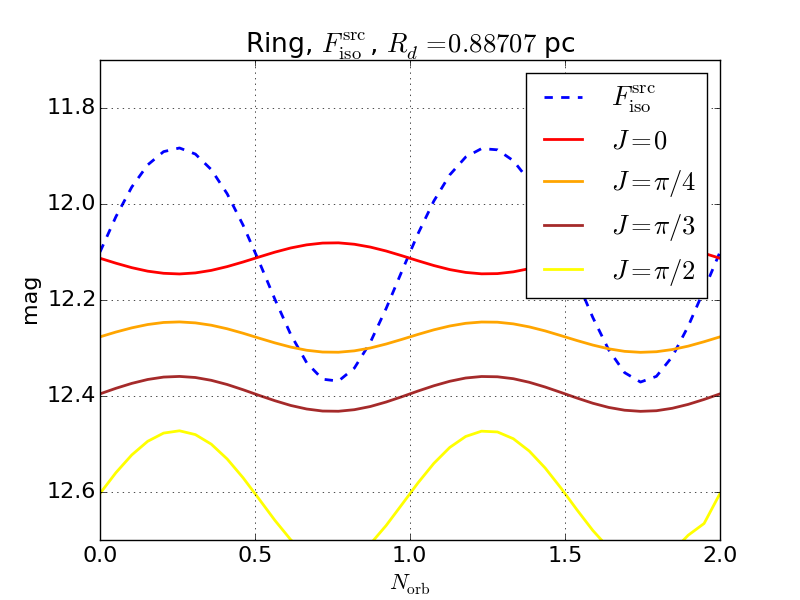
\includegraphics[scale=0.27]{figures/Ring/FISO_Ring_nrm-9p32812__Rin2p73218e+18_VaryJ_numin1e-05_numx100} &
% 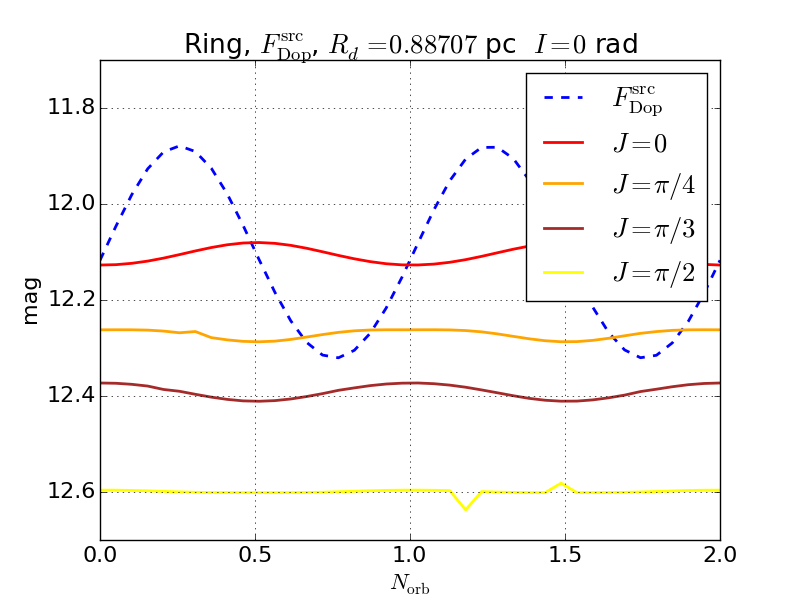
\includegraphics[scale=0.27]{figures/Ring/FDop_Ring_nrm-9p32931__Rin2p73218e+18_Inc0_VaryJ_numin1e-05_numx100} &
% 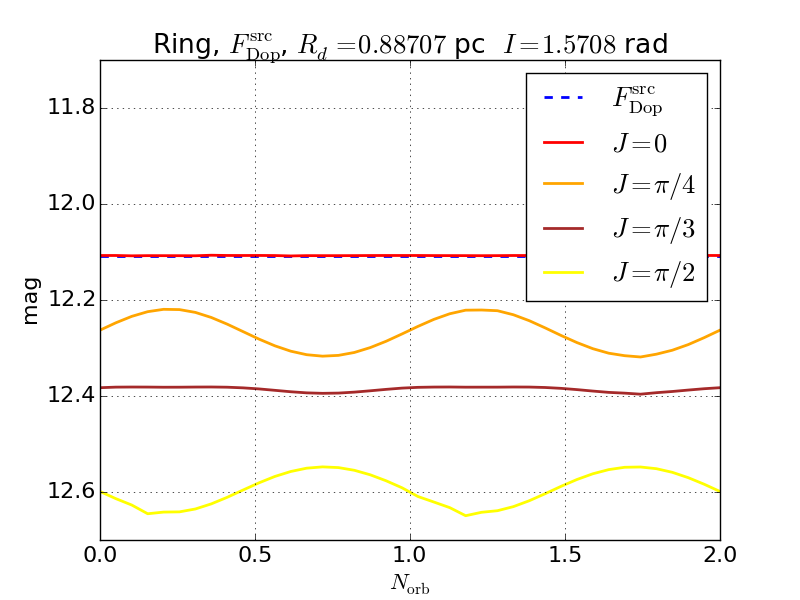
\includegraphics[scale=0.27]{figures/Ring/FDop_Ring_nrm-9p33301__Rin2p73218e+18_Inc1p5708_VaryJ_numin1e-05_numx100} 
% %
% \end{array}$
% \end{center}
% \caption{Rings}
% \label{Fig:Rd}
% \end{figure}
% %%%%%%%%%%%%%%%%%%%%%%%%%%%%%%%%%%%%%%%%%%%%%%%%















\subsection{Torus Shell} 
Figures \ref{Fig:ShTor1} and \ref{Fig:ShTor2} plot IR emission from an
infinitely thin dust torus with opening angle $\theta_T$ and inclination to
the line of sight $J$. The top rows assumes that the dust is optically thin to
it own emission as before, while the bottom row assumes the opposite, that IR
emission is blocked when any part of the torus shells lies between the observer
and emission source.

The top row of \ref{Fig:ShTor1} shows that rotation of the dust torus alone
can shift the phase of the reprocessed emission by an entire cycle. This is
because rotating the torus changes where the majority of IR emission emanates
from by a factor of $\sim \Rin$. For the narrower $\theta_T$ in Figure
\ref{Fig:ShTor2} this effect is reduced.



The bottom row of Figure \ref{Fig:ShTor1} shows the effect of blocking out IR
emission. The obscured $J=0$ (red) and $J=\pi/2$ (yellow) models are too dim
to be plotted. Only the partially obscured $J=(\theta_T - \pi/2)/2$ (orange)
and $J=(\theta_T - \pi/2)/$ (brown) are bright enough to be observed. For the
smaller torus opening angle in Figure \ref{Fig:ShTor2}, even less IR emission
escapes.





%%%%%%%%%%%%%%%%%%%%%%%%%%%%%%%%%%%%%%%%%%%%%%%%
%%% FIGURE: Opt Thin and Thick Torus Shells ISO vs Dop%%%
%%%%%%%%%%%%%%%%%%%%%%%%%%%%%%%%%%%%%%%%%%%%%%%%
\begin{figure}
\begin{center}$
\begin{array}{c c}
%FISO and DOP  vary Rin
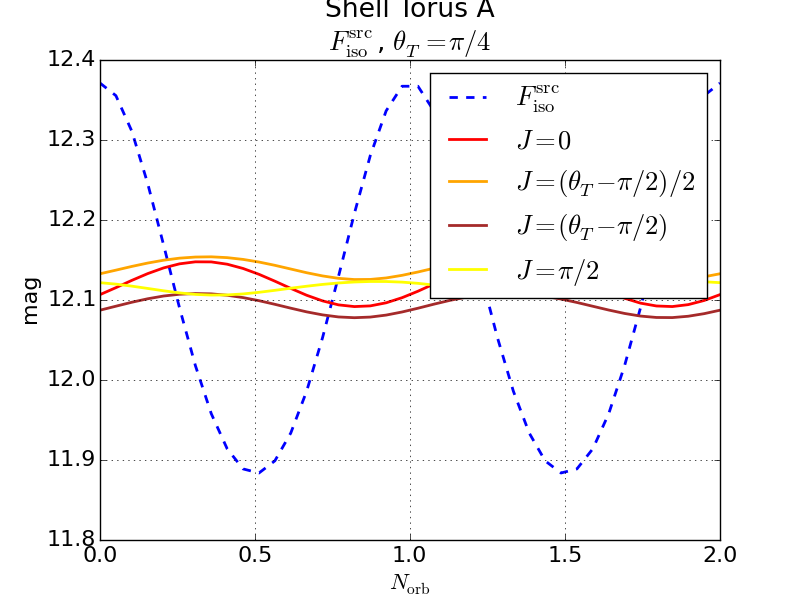
\includegraphics[scale=0.27]{figures/ch5/ShTor_Thin/FISO_ShTor_Thin_nrm1p352__Rin2p73218e+18_Inc0_thetaT0p785398_VaryJ_numin1e-05_numx100} & 
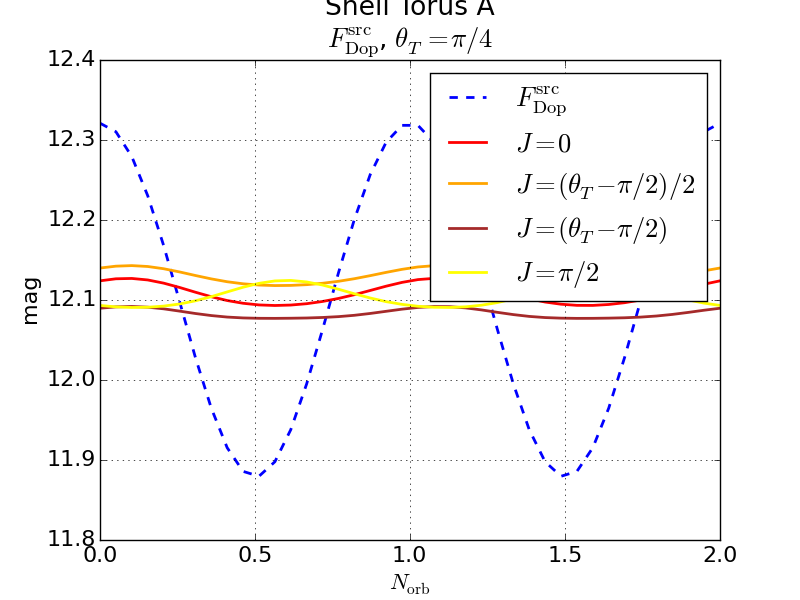
\includegraphics[scale=0.27]{figures/ch5/ShTor_Thin/FDop_ShTor_Thin_nrm1p34412__Rin2p73218e+18_Inc0_thetaT0p785398_VaryJ_numin1e-05_numx100} \\
%
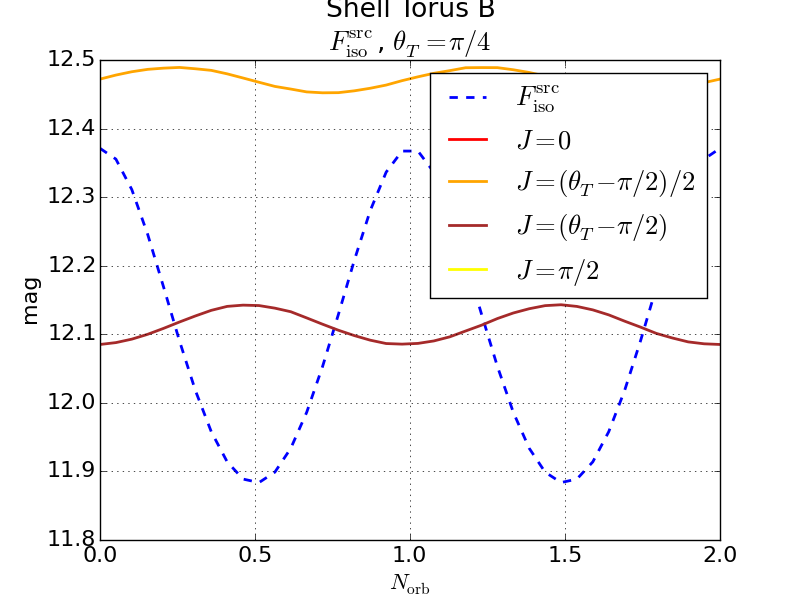
\includegraphics[scale=0.27]{figures/ch5/ShTor_Thick/FISO_ShTor_Thick_nrm0__Rin2p73218e+18_Inc0_thetaT0p785398_VaryJ_numin1e-05_numx100} & 
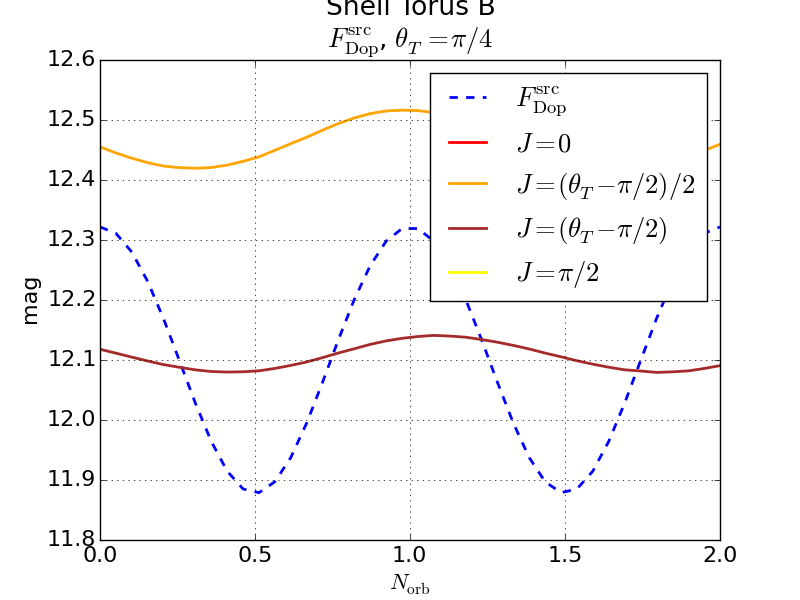
\includegraphics[scale=0.27]{figures/ch5/ShTor_Thick/FDop_ShTor_Thick_nrm0__Rin2p73218e+18_Inc0_thetaT0p785398_VaryJ_numin1e-05_numx100} 
\end{array}$
\end{center}
\caption{Geometrically thin torus dust shells - very optically thick to optical/UV. The top row shows the difference in isotropic vs. Doppler boost models for an optically thin to IR model. The bottom row shows the same for a model in which dust blocks the emitted IR. The UV/optical emission (dashed) is displayed without absorption.}
\label{Fig:ShTor1}
\end{figure}
%%%%%%%%%%%%%%%%%%%%%%%%%%%%%%%%%%%%%%%%%%%%%%%%





%%%%%%%%%%%%%%%%%%%%%%%%%%%%%%%%%%%%%%%%%%%%%%%%
%%% FIGURE: Opt Thin and Thick Torus Shells ISO vs Dop%%%
%%%%%%%%%%%%%%%%%%%%%%%%%%%%%%%%%%%%%%%%%%%%%%%%
\begin{figure}
\begin{center}$
\begin{array}{c c}
%FISO and DOP  vary Rin
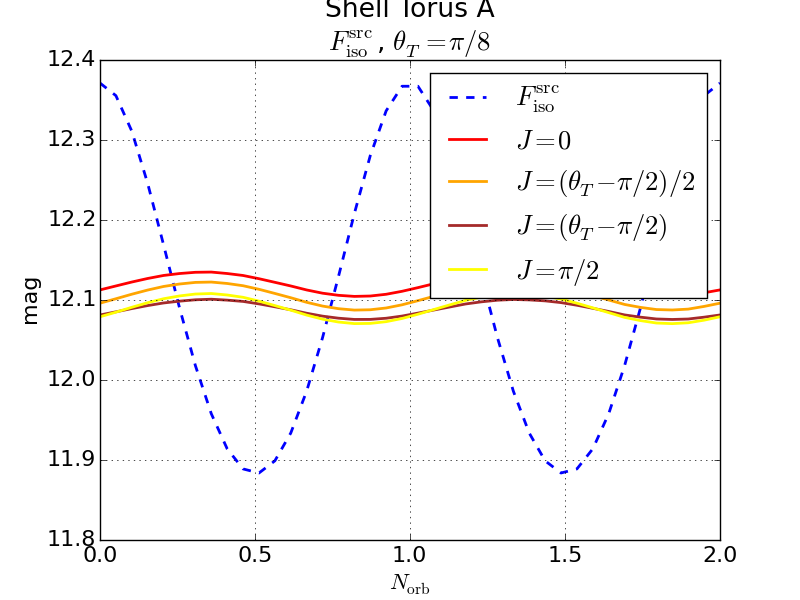
\includegraphics[scale=0.27]{figures/ch5/ShTor_Thin/FISO_ShTor_Thin_nrm2p07131__Rin2p73218e+18_Inc0_thetaT0p392699_VaryJ_numin1e-05_numx100} & 
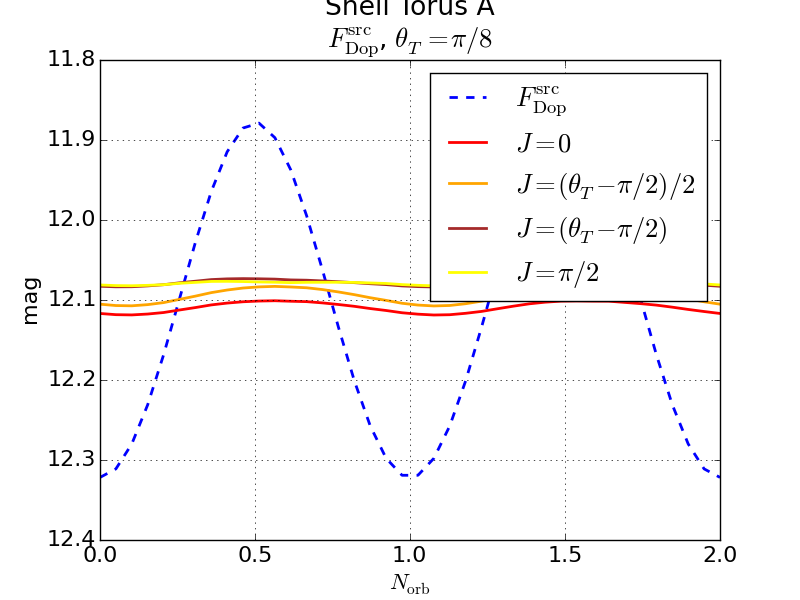
\includegraphics[scale=0.27]{figures/ch5/ShTor_Thin/FDop_ShTor_Thin_nrm2p06282__Rin2p73218e+18_Inc0_thetaT0p392699_VaryJ_numin1e-05_numx100} \\
%
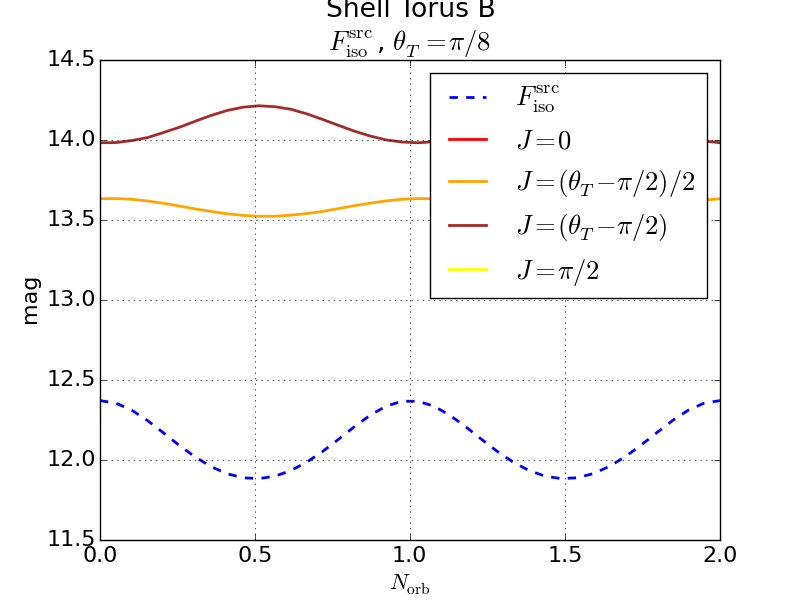
\includegraphics[scale=0.27]{figures/ch5/ShTor_Thick/FISO_ShTor_Thick_nrm0__Rin2p73218e+18_Inc0_thetaT0p392699_VaryJ_numin1e-05_numx100} & 
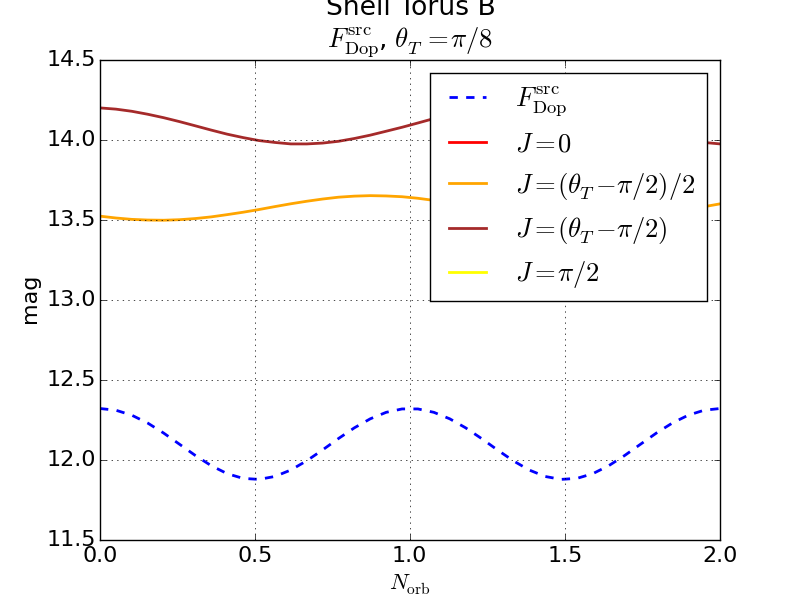
\includegraphics[scale=0.27]{figures/ch5/ShTor_Thick/FDop_ShTor_Thick_nrm0__Rin2p73218e+18_Inc0_thetaT0p392699_VaryJ_numin1e-05_numx100} 
\end{array}$
\end{center}
\caption{The same as Figure \ref{Fig:ShTor1} but for a smaller torus opening angle.}
\label{Fig:ShTor2}
\end{figure}
%%%%%%%%%%%%%%%%%%%%%%%%%%%%%%%%%%%%%%%%%%%%%%%%







\subsection{Torus with finite radial extent}
%Figure \ref{Fig:TorThick} shows the IR emission from the a torus with finite extent for which optical and UV emission penetrates into the dust until it fully absorbed. We choose to integrate out to the radius where the optical depth to UV/optical is $3$. The dust is assumed optically thin to its own emission and is free to escape. Each panel chooses a $1/r^2$ fall off in dust number density with radius and varies the density normalization. 

This IR light curves from this model depend on the dust density distribution through the normalization $n_0$ and the power law exponent of radial fall off. These two set the outer limit of IR emission and also the average brightness of the IR light curves. Though this case is still under investigation, we do find that the choice of the outer limit of integration is important. The best choice is at a radius where $r>R_{\tau=1}$. Above a certain density, we find that the brightness limits to its maximum value.



% %%%%%%%%%%%%%%%%%%%%%%%%%%%%%%%%%%%%%%%%%%%%%%%%
% %%% FIGURE: Opt Thin and Thick Torus Shells ISO vs Dop%%%
% %%%%%%%%%%%%%%%%%%%%%%%%%%%%%%%%%%%%%%%%%%%%%%%%
% \begin{figure}
% \begin{center}$
% \begin{array}{c c}
% %FISO and DOP  vary Rin
% 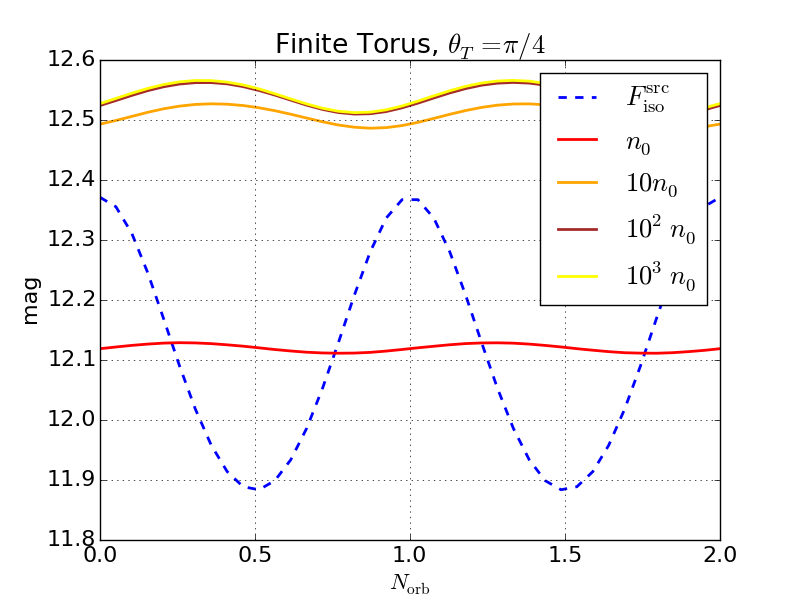
\includegraphics[scale=0.27]{figures/ch5/Thick_OptThin/FISO_TorThick_OptThin_nrm1p47494__Rin2p73218e+18_Inc0_J0_thetaT0p785398_Varyn0_numin1e-05_numx100} & 
% 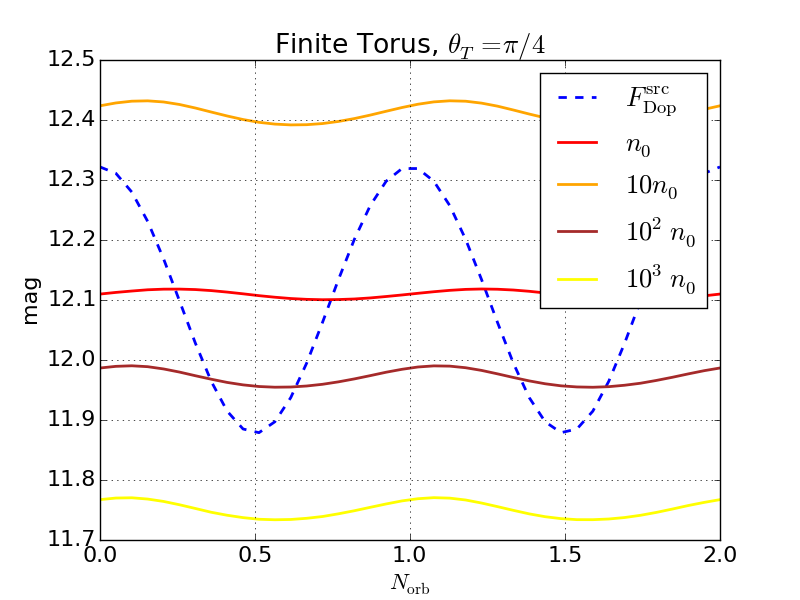
\includegraphics[scale=0.27]{figures/ch5/Thick_OptThin/FDOP_TorThick_OptThin_nrm1p46962__Rin2p73218e+18_Inc0_J0_thetaT0p785398_Varyn0_numin1e-05_numx100} 
% \end{array}$
% \end{center}
% \caption{Geometrically thick, optically thin tori. Left and right panels show the difference between isotropic vs. Doppler boost models, for varying dust density normalization $n_0$.}
% \label{Fig:TorThick}
% \end{figure}
% %%%%%%%%%%%%%%%%%%%%%%%%%%%%%%%%%%%%%%%%%%%%%%%%











\section{The case of PG 1302}
\label{S:PG1302}
We now apply our model to the periodically variable quasar PG 1302-102. We use data published by J15 from the W1 and W2 band of the WISE instrument at $3.4 \mu$m ($2.8 \rightarrow 4.0 \mu$m) and $4.6 \mu$m ($3.9 \rightarrow 5.3 \mu$m) respectively. The longer wavelength WISE W3 ($12 \mu$m) and W4 ($22 \mu$m) bands are not reported because these bands only took data during the cryogenic phase of the WISE mission (before it ran our of coolant circa late 2010) and the data is too sparse to be useful for period recovery (see J15)\footnote{The W3 and W4 data, even if only at one epoch, would be useful constraints on PG 1302's SED. Future model fitting should include this data}. Data for W1 and W2 however exists at 6 month intervals from 2010 to July 2015 with a three year gap during hibernation between 2011 and 2014. Each set of measurements is made up by $\sim 10$ measurements taken within a few days of each other. We average these $\sim10$ measurements and use a single data point with gaussian propagated errors at each 6 month interval. %Figure \ref{Fig:sinfit} shows the averaged data points with errors in black overlaid with all of the data in color. Figure \ref{Fig:sinfit} also shows the best fit sinusoids to the data (dashed lines).


For all model fitting we minimize a simple $\chi^2$ likelihood.
To characterize the IR data, we fist perform fit of three different sinusoids to the optical, W1, and W2 data.
From fitting sinusoids to the W1 and W2 light-curves, while fixing the observed period at $1884$ days, we find that in addition to a phase lag, the observed variability amplitude of the infrared data is $56\pm5\%$ (W1) and $63\pm5\%$ (W2) of the optical variability amplitude. We find maximum likelihood values for the phase lag of $534\pm13$ days and $600\pm13$ days for W1 and W2 respectively, consistent with, but at larger values than the results of J15.  Details are found in the Appendix.


Our main goal is compare the dust reverberation models when using Doppler
boosted central source variability, vs. variability from an isotropically varying central source.
To fit the dust models, we to first find the
best fit to the optical data and use these as input to fit the
dust reverberation models to the WISE data. Because the amplitude of the source variability 
need not be that of the optical, we fit also for $\alpha$ in the Doppler boost 
model, and the amplitude $A$ in the isotropic emission model. This is 
simply parameterizing our ignorance of the spectrum of variability across the optical 
and UV wavelengths. We may check for consistency with known FUV and NUV amplitudes a posteriori.


We present the result of fitting the final model of \S \ref{S:ThickTor}, a dust torus 
optically thick to UV radiation, but optically thin to
IR radiation. In this case, the UV/optical emission heats up an inner region 
of the dust torus and the IR radiation escapes freely. 
The size of the emitting region is set by the dust density distribution. 
Table \ref{Table:Fit} displays our best fit parameters for PG 1302 using both an 
isotropic and a Doppler boosted central source. We find preliminarily that both models 
of IR reverberation can fit the data, but this must be confirmed and tested with other dust models. 

It is interesting to note that the best fit dust tours obscures the central source. This is not consistent with the smooth dust medium employed here, but a clumpy medium would allow a portion of UV light through.




To understand the parameter dependencies and
constraints that our model places on them, we are currently running a Markov
Chain Monte Carlo analysis using the publicly available code \textsc{emcee} \citep{DFM:2013}. Fitting using other dust models is also a work in progress.

We note one caveat: in the fits displayed in Figure \ref{Fig:Fit1}, IR emission is integrated from the best fit inner dust shell edge out to $R_{\tau=1} + 0.01 \Rin$. The dependence on the outer radius of integration is currently being investigated. A full analysis of best fit parameters, their uncertainties, and model selection is pending


%%%%%%%%%%%%%%%%%%%%%%%%%%%%%%%%%%%%%%%%%%%%%%%%
%%% FIGURE: Bet fits ISO vs Dop%%%
%%%%%%%%%%%%%%%%%%%%%%%%%%%%%%%%%%%%%%%%%%%%%%%%
\begin{figure}
\begin{center}$
\begin{array}{c c}
%FISO and DOP  
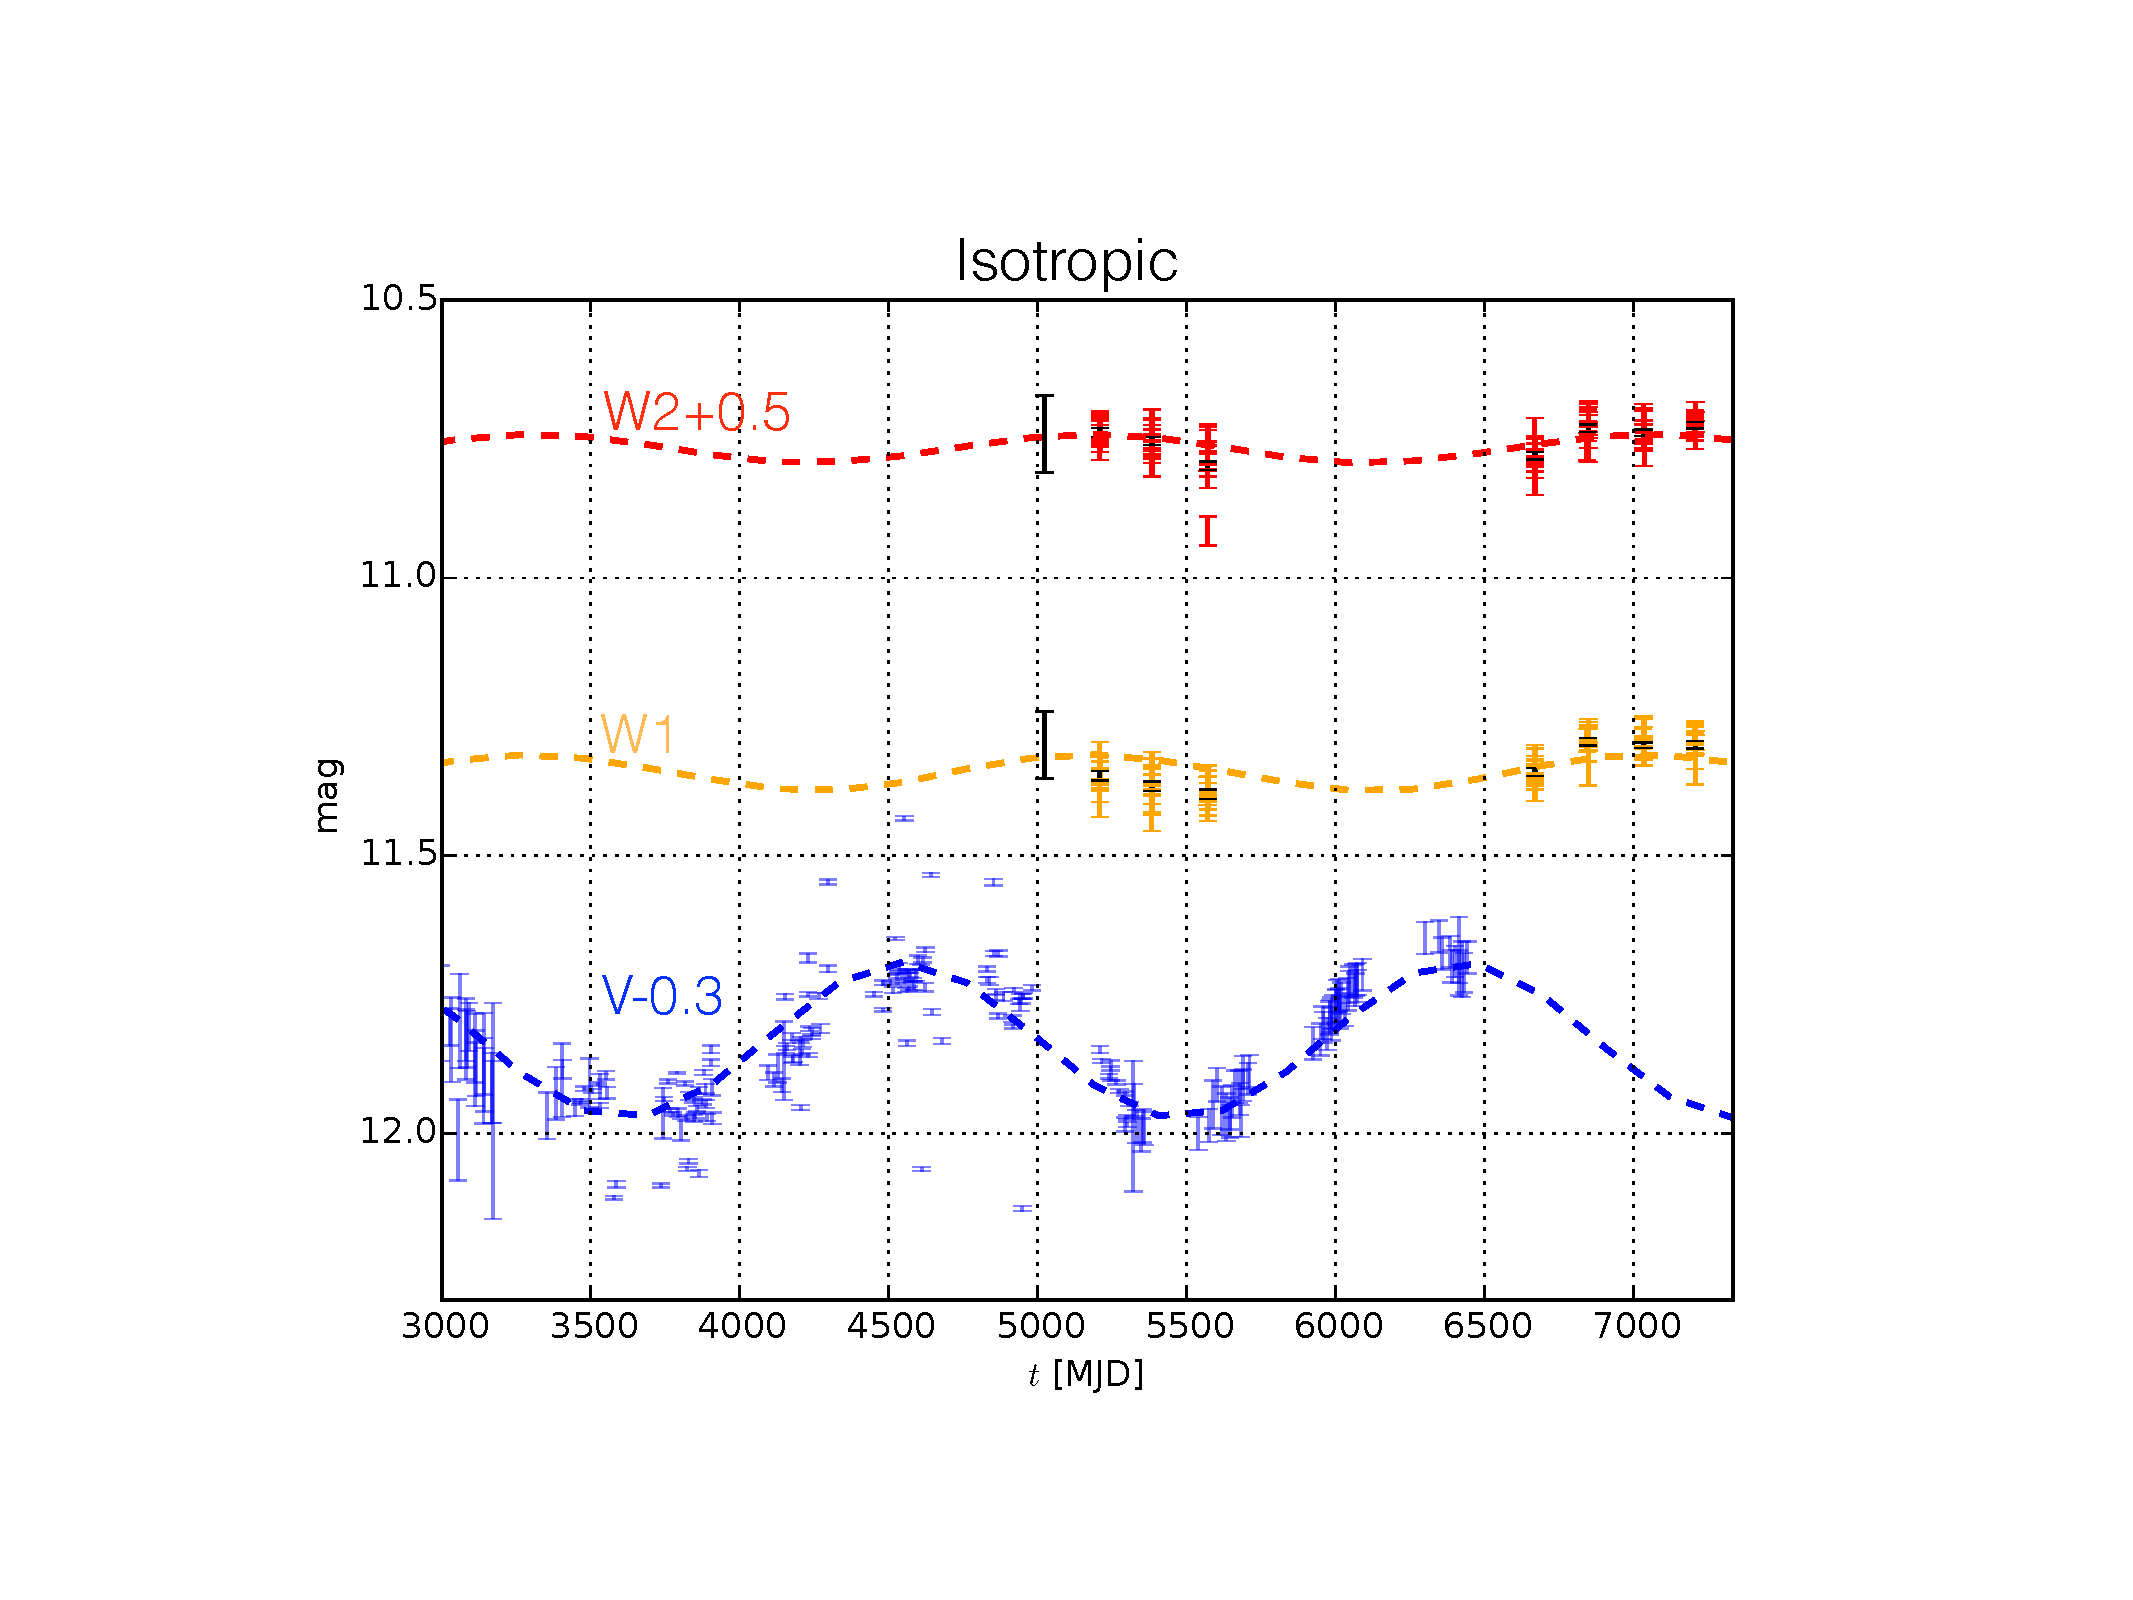
\includegraphics[scale=0.27]{figures/ch5/Fitting/ISO_Best_fit_Case3_Labels} & 
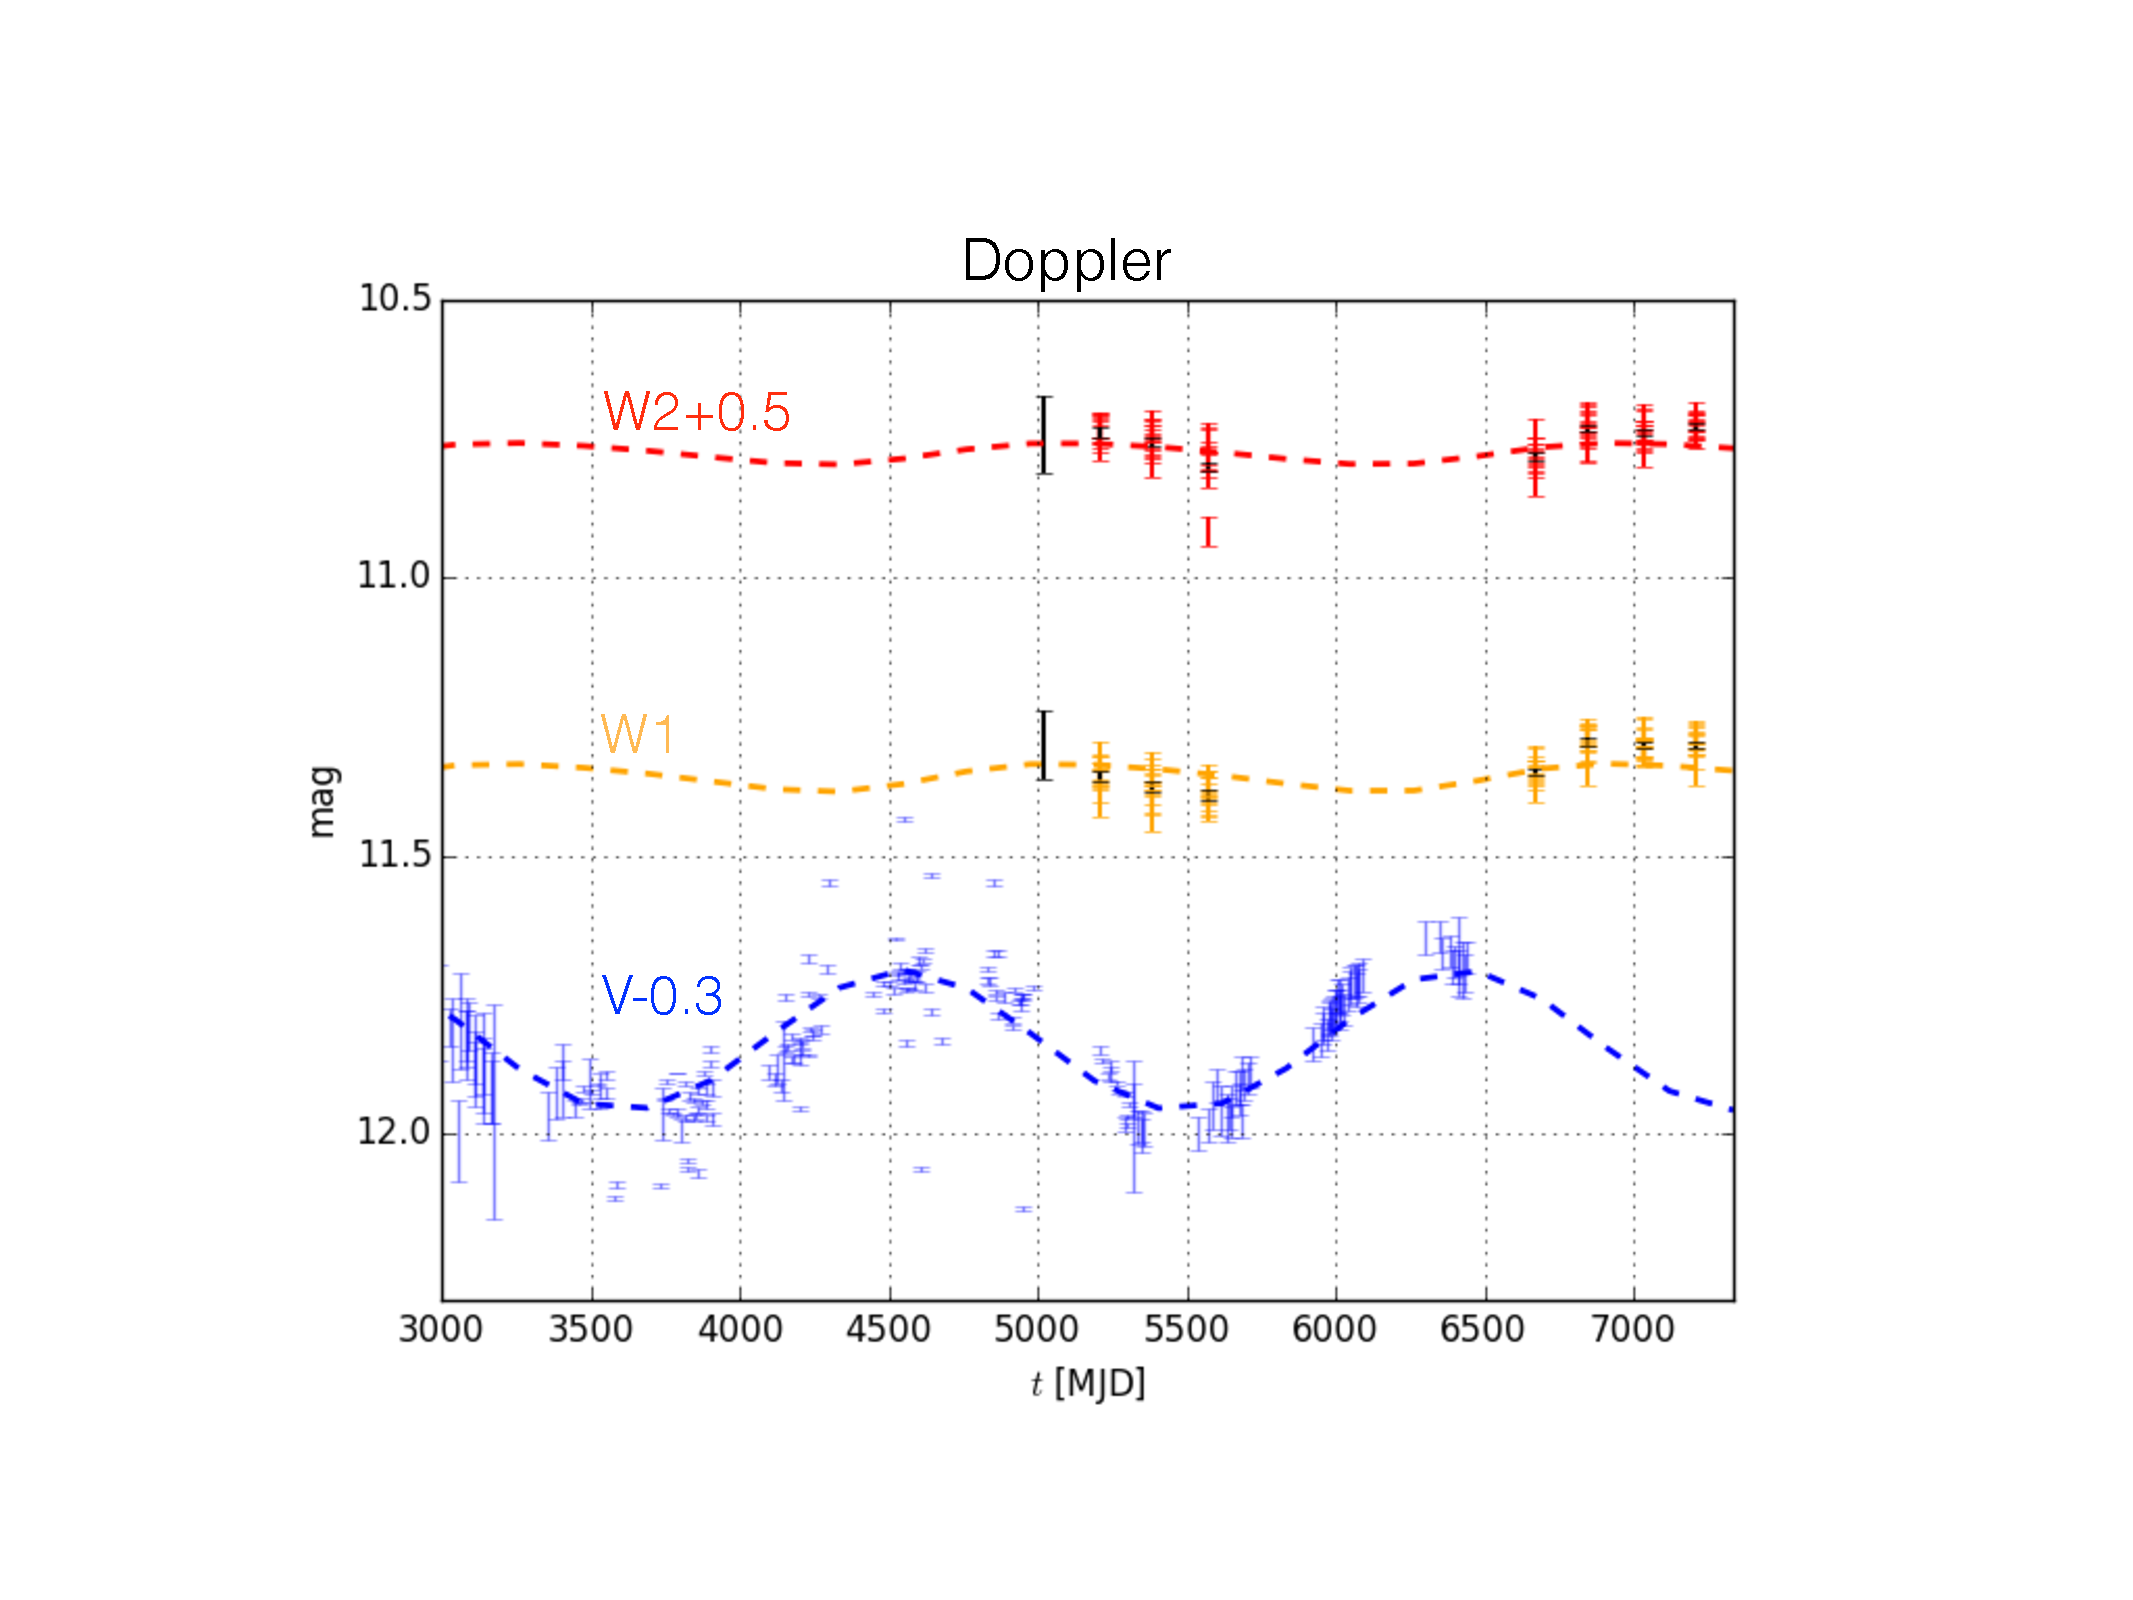
\includegraphics[scale=0.27]{figures/ch5/Fitting/Dop_Best_fit_Case3_Labels} 
\end{array}$
\end{center}
\caption{PRELIMINARY: The best fit isotropic source and Doppler boosted source light curves. A full analysis of best fit parameters, their uncertainties, and model selection is pending}
\label{Fig:Fit1}
\end{figure}
%%%%%%%%%%%%%%%%%%%%%%%%%%%%%%%%%%%%%%%%%%%%%%%%




% \begin{table}
% \begin{center}
% \begin{tabular}{ c |     c | c  |c }
% Parameter               &                  				 & PG 1302 value    &  \\
%                    \hline 
% Binary Parameters  &  Opt. Thin Shell Torus        & Opt. Thick Shell Torus &  Opt. Thin Torus  \\
%                   \hline		
% $\Omega$               &$2 \pi / 1474$ days  			 &"                            & "   \\
% $\beta$		       & 0.8		   				 &"		   	       & "  \\
% $I$                           &  $\cos^{-1}{(0.067/\beta)}$    	 &"		   	       & "  \\
% $\bar{\alpha}$          &  -2.0  				   	 &"		   	       & "  \\ 
%                    \hline 	
%                   Dust Parameters & \\
%                   \hline	
% \textcolor{green}{$\Rin$}            & $0.9 \sqrt{\epsilon/0.1}$ pc            	  & $0.9 \sqrt{\epsilon/0.1}$ pc  		  & $0.9 \sqrt{\epsilon/0.1}$ pc \\
% \textcolor{green}{$n_0$}            & ? $(p-1) (\pi a^2_{\eff} \Rin)^{-1}$	  & ? $(p-1) (\pi a^2_{\eff} \Rin)^{-1}$   & ? $(p-1) (\pi a^2_{\eff} \Rin)^{-1}$	\\
% \textcolor{green}{$p$}              	& ?						        	  & ?							  & ?	\\
% \textcolor{green}{$J$}              	& ?						        	  & ?							  & ?	\\
% \textcolor{green}{$\theta_T$}   	& ?						        	  & ?							  & ?	\\
% $\Rout$                                  	& $10\Rout$ 				           &"		   	    				  & "  \\
% $k$		    			  	&  1 							  &"		   	    				  & "  \\
% $\nu_0$					&  $c/(2 \pi a_{\rm{eff}})$			  &"		   	    				  & "  \\
% $a_{\rm{eff}}$		         	& $0.16$ $\mu$m				  &"		   	    				  & "  
%  \end{tabular}
% \caption{Maximum likelihood parameters for three different dust models for PG 1302.} %Those colored green are allowed to vary in a model fit to infrared data from PG 1302}
% \label{Table:Fit}
% \end{center}
% \end{table}




\begin{table}
\begin{center}
\begin{tabular}{ l |     c | c  |c }
%              &                  				 & PG 1302 value    &  \\
  %                 \hline 
Doppler Source        				& Isotropic Source  				&  \\
                  \hline				
$P =  1464$ days  				 & $P =  1464$ days  			 & \\
$\beta = 0.068$		   			 & \textcolor{green}{$A $}$= 0.38$	& \\
$t_0 = 0.66P$  					&  $t_0 = 0.69P$		   	         & \\ 
$I = 0.02^{\circ}$  				& 		   	       				&\\ 
\textcolor{green}{$\alpha$}$ = -2.0$  & 	   	   					 &\\
                   \hline 	
                  Dust Parameters &   &\\
                  \hline	
\textcolor{green}{$J$}              	& $41^{\circ}$					  & $42^{\circ}$				  	\\
\textcolor{green}{$\theta_T$}   	& $18^{\circ}$					  & $15^{\circ}$							  	\\
\textcolor{green}{$\Rin$}            & $6.0$ pc            				  & $6.0$ pc					  		   \\
\textcolor{green}{$n_0$}            &  $1.24 \times 10^{-7}$ cm$^{-3}$	  & 1.26$ \times 10^{-7}$ cm$^{-3}$   	\\
%\textcolor{green}{$n_0$}            & ? $(p-1) (\pi a^2_{\eff} \Rin)^{-1}$	  & ? $(p-1) (\pi a^2_{\eff} \Rin)^{-1}$   	\\
%$R_{\tau=1}$                              & $0.1$ pc 				           & ? 		   	    				    \\
$p$   			           	& 2						        	  & "							  	\\
$k$		    			  	&  1 							  &"		   	    				    \\
$a_{\rm{eff}}$		         	& $0.24$ $\mu$m				  &"	\\
$\nu_0$					&  $c/(2 \pi a_{\rm{eff}})$			  &"		   	    				    \\
\hline
%$\chi^2/\nu$			        &  15		 					 & 18		   	    				    \\

 \end{tabular}
\caption{Maximum likelihood parameters for three different dust models for PG 1302. A full analysis of best fit parameters, their uncertainties, and model selection is pending. Parameters colored green are allowed to vary.}
\label{Table:Fit}
\end{center}
\end{table}








\section{Discussion}
\label{S:Discussion}
As this is ongoing work, we list now only caveats and possible extensions to this work.

\subsection{Caveats and Possible extensions to the Toy Model}
\begin{itemize}
\item \textbf{Dust tori are thought to be clumpy:} This may be added to our model with a more complicated dust density. %If the dust is clumpy we would expect larger amplitude modulations in the IR light curves predicted by this model. This is because modulation is enhanced by non-uniform reprocessing of the continuum. That is, a uniform sphere of dust should exhibit the lowest amplitude IR light curves. 
%
\item \textbf{Dust grain size distribution:} We have assumed a uniform distribution of dust grain sizes. In reality there will be a distribution of dust grain species and sizes. %may be a gradient in radius due to the radial gradient in dust temperature and density.
%
\item \textbf{Relative location of central source:} We have argued that the relative location of the emitting secondary is small compared to the dust torus inner radius. A model where this is taken into account will be important for modeling the effects of Doppler boosted emission on broad line regions around MBHBs and will be the subject of a companion paper.
%
\item \textbf{Circular binary:} Some hydrodynamical models of the binary interaction with a gas disk predict that large binary eccentricities can be excited \citep{Roedig:2011:eccevo}. Such binary eccentricities will change the shape of the optical and hence the IR light curves predicted here. 
%
%(though for near equal mass binaries for which eccentricities where Doppler boosting may not be as important)
%
\item \textbf{Scattering and line emission:} We have assumed for simplicity that continuum photons are only absorbed and heat up the dust and that  emitted photons are only absorbed by line of sight dust. In actuality scattering and line emission could be important and also useful as observational diagnostics of the dust environment.
%\item{\textbf{AGN unification:} Because the models here predict the relative inclination of the dusty torus, they can be tested within the AGN unification model.}

\item \textbf{Motion of binary relative to the dust:} Because of finite light travel times, the relative motion of the binary with respect to the dusty torus will become important on the level of the ratio of the binary separation and the size of the infrared reprocessing region (the dust). The ratio of binary separation to torus inner edge is
\begin{equation}
\frac{a}{R_d} \simeq 0.016\ \epsilon_{0.1} \left(\frac{M}{10^9 \Msun}\right)^{-1/6}  \left(\frac{P}{5 \rm{yr}}\right)^{2/3}  \left(\frac{T}{1800 \rm{K}}\right)^{2.6}.
\label{Eq:aORd}
\end{equation}
This ratio tells us the impact of binary orbital motion on the time lags of reprocessed light will be most important for the lowest mass binaries with the longest periods and contribute on at at most the $1.6 \%$ level for the fiducial values taken here for a PG1302-like binary. Because the dependence on mass is weak, and 5 years is a current upper limit on observed binary periods discovered in EM time-domain surveys \citep[\textit{e.g.}][]{Graham+2015b}, it is safe to assume that the effect of binary orbital motion is a $\lsim 2\%$ effect.% and we ignore it for the remainder of this work, assuming that the binary emission comes from the center of coordinates throughout. We plan to incorporate the effect of changing binary orbital position in future work on broad emission lines, in which case the binary separation is a larger fraction of the broad line region.
 %
 \item \textbf{General relativistic time lags and precession:} could also become important. %http://arxiv.org/abs/1604.02148
 %
 \item \textbf{A changing dust sublimation radius:} If grains can re-form on a timescale shorter than a binary orbital time, the inner sublimation radius will change periodically with the changing central source flux. From Eq. \ref{Eq:Rd}, the change in dust sublimation due to the changing observed flux variations $\delta F$ is
 \begin{equation}
 \frac{\delta R_d}{R_d} = \frac{1}{2} \frac{\delta F}{F}
 \end{equation}
which could result in changes to the inner dust radius of a few to $\sim 10 \%$ for typical Doppler flux variations.
\end{itemize}


\section{Conclusions}
We have developed a model to compute IR light curves from isotropically emitting and anisotropically emitting Doppler boosted MBHBs. The latter, describing reverberation from a lighthouse-like central source is presented here for the first time. We show that the phase, amplitude, and brightness of reverberated IR radiation is dependent not only on the physical size of the reverberation region, but can be equally influenced by the dust geometry, variability timescale relative to the dust size, and in the case of Doppler boosted emission, the relative inclination of binary orbital plane and dust torus. This model can be used to interpret the nature of the growing list of MBHB candidates, and their surrounding dust regions, by interpreting their IR emission; though we have not yet concluded whether IR emission from a Doppler boosted source will be discernible from an isotropically varying source.


This model will not only be useful for interpreting the nature of existing candidates but could help to discover more. If the binary's orbit is highly inclined to the line of sight, but not to the dust structure, then an imprint of Doppler boosting will not appear in the optical and UV, but it will appear in the IR. This motivates a search for any such concealed Doppler imprints in the IR.

Finally we have fit a dust model to the MBHB Doppler boost candidate PG 1302. We find agreement across the W1 and W2 wise bands, but have not yet discerned wether such a dust model rules out an isotropically varying source vs. the Doppler boost model.

%Our main results are...
%\begin{enumerate}
%\item The phase lag of the IR curve is dependent not only on the size of the emission region, but also on the geometry and orientation of the dust torus as well as the relative pattern speed of the variable illuminating source...allowing IR and optical/UV data to constrain dust and binary parameters. 
%\item Assuming binary parameters found from fits to the optical and UV data, our model makes predictions consistent with the measured IR light curves for PG 1302 (J15). The best fit dust parameters are given in Table \ref{Table:Fit}. 
%\item Even if UV/optical modulation is not visible because of near face on binary orbital inclinations, the IR modulation could still be observable depending on the relative inclination of the dust torus. Periodicity searches in IR surveys such as WISE could find a population of highly-inclined MBHB candidates as well as provide evidence for (or against) existing MBHB candidates that exhibit periodic optical and IR data.
%\end{enumerate}



%\section{Acknowledgments}


\appendix
\section{MCMC fits}
\subsection{Sinusoid Fit}
%From fitting sinusoids to the W1 and W2 light-curves, while fixing the observed period at $1884$ days, we find that in addition to a phase lag, the observed variability amplitude of the infrared data is $56\pm5\%$ (W1) and $63\pm5\%$ (W2) of the optical variability amplitude. We find maximum likelihood values for the phase lag of $534\pm13$ days and $600\pm13$ days for W1 and W2 respectively, consistent with, but at larger values than the results of J15.
The best sinusoid fits to the PG1302 optical and IR data using a Monte Carlo Markov Chain algorithm \citep{DFM:2013}.


%%%%%%%%%%%%%%%%%%%%%%%%%%%%%%%%%%%%%%%%%%%%%%%%
%%% FIGURE: Sin Fits %%%
%%%%%%%%%%%%%%%%%%%%%%%%%%%%%%%%%%%%%%%%%%%%%%%%
\begin{figure}
\begin{center}$
\begin{array}{c c c}
%
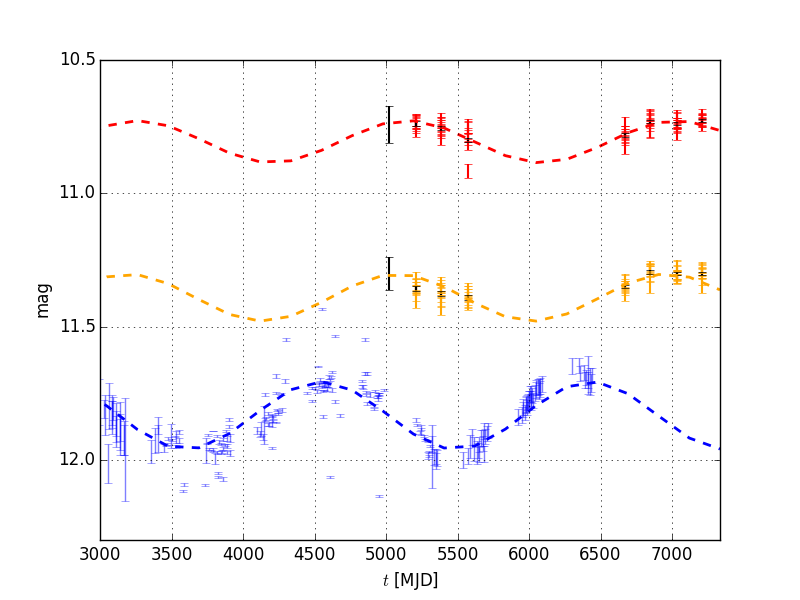
\includegraphics[scale=0.33]{figures/ch5/Sin_MCfit/SinFit_NOPrdBestFit}  \\
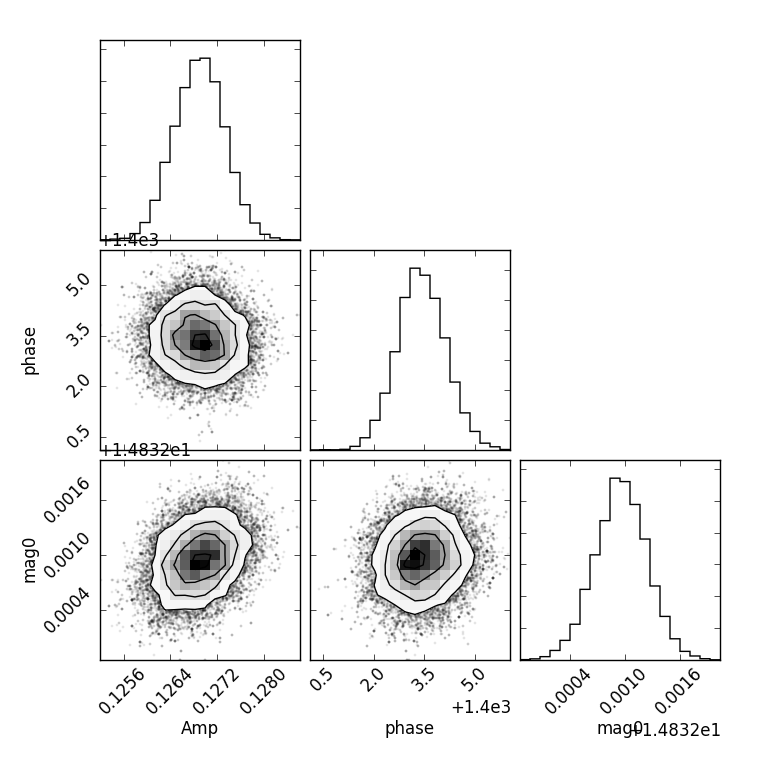
\includegraphics[scale=0.2]{figures/ch5/Sin_MCfit/Fsrc_PG1302_Corner_Plot_2048walkers}& \hspace{-30pt}
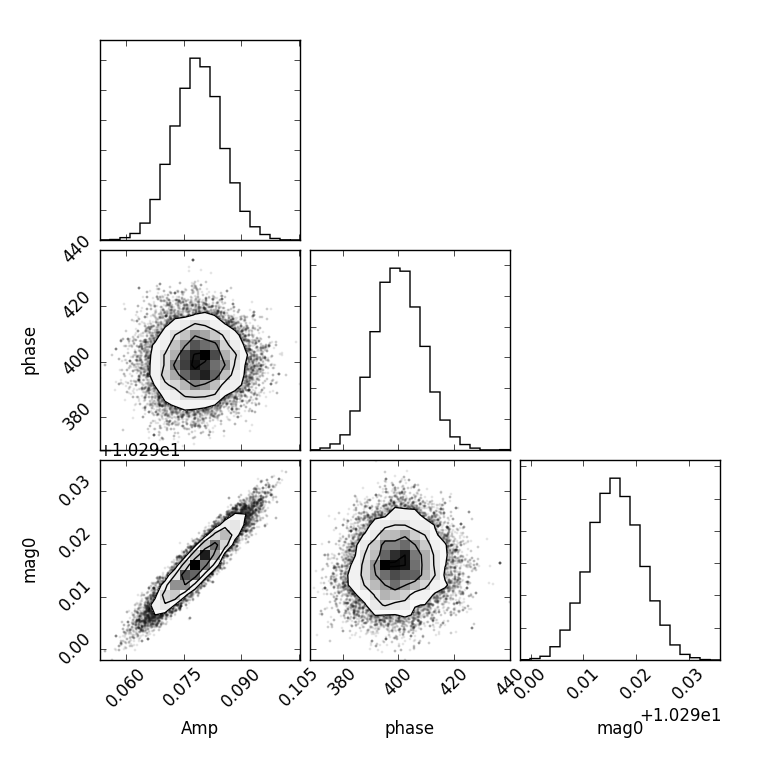
\includegraphics[scale=0.2]{figures/ch5/Sin_MCfit/W2_sin_PG1302_Corner_Plot_2048walkers}&
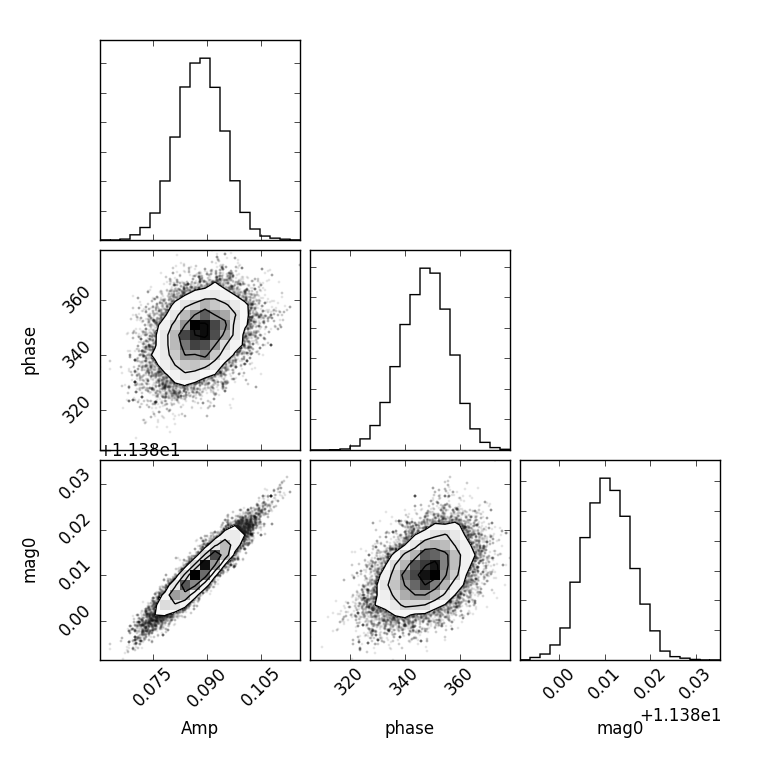
\includegraphics[scale=0.2]{figures/ch5/Sin_MCfit/W1_sin_PG1302_Corner_Plot_2048walkers}
%
\end{array}$
\end{center}
\caption{Left: Best fit sin models. Right: Corner plot for 2048 steps by 48 walkers showing parameter correlations and posterior distributions.}
\label{Fig:ShellFit}
\end{figure}
%%%%%%%%%%%%%%%%%%%%%%%%%%%%%%%%%%%%%%%%%%%%%%%%


































































%\bibliographystyle{mnras}
%\bibliography{refs}

%\end{onecolumn}
%\end{document}


\renewcommand\thesection{\thechapter.\arabic{section}}